% CSE 4112 Dataset Report — follows report/CSE_4112_Dataset_Report_Template.docx section by section.
% Build:  cd report ; ..\venv\Scripts\python.exe build_report_assets.py ; latexmk -xelatex CSE_4112_Dataset_Report.tex
\documentclass[11pt,a4paper]{article}

% ---------------------------------------------------------------- page, fonts, spacing (template: A4, ~20 mm, TNR 11 pt, Arial headings, 1.15, 6 pt after)
\usepackage[a4paper,margin=20mm,headheight=14pt]{geometry}
\usepackage{fontspec}
\setmainfont{Times New Roman}
\setsansfont{Arial}
\usepackage{amsmath,amssymb}
\usepackage{setspace}
\setstretch{1.15}
\setlength{\parindent}{0pt}
\setlength{\parskip}{6pt}
\usepackage[table]{xcolor}
\usepackage{graphicx,array,tabularx,longtable,multirow,booktabs,float,enumitem,fancyhdr,titlesec,caption,subcaption,fancyvrb}
\usepackage[section]{placeins}
\makeatletter
\setlength{\@fptop}{0pt}\setlength{\@fpsep}{12pt}\setlength{\@fpbot}{0pt plus 1fil}
\makeatother
\usepackage{tikz}
\usetikzlibrary{arrows.meta,positioning,calc}
\usepackage[hidelinks]{hyperref}
\usepackage{xurl}

\definecolor{diag}{HTML}{DBEAF7}
\definecolor{qhead}{HTML}{EEF1F4}
\definecolor{hdr}{HTML}{F2F2F2}
\definecolor{accent}{HTML}{2A78D6}

\titleformat{\section}{\sffamily\bfseries\large}{}{0pt}{}
\titleformat{\subsection}{\sffamily\bfseries\normalsize}{}{0pt}{}
\titleformat{\subsubsection}{\sffamily\bfseries\small}{}{0pt}{}
\titlespacing*{\section}{0pt}{10pt}{2pt}
\titlespacing*{\subsection}{0pt}{8pt}{1pt}
\titlespacing*{\subsubsection}{0pt}{6pt}{0pt}

\captionsetup{font={small,sf},labelfont=bf,labelsep=period,justification=justified,singlelinecheck=true}
\captionsetup[table]{position=top,skip=3pt}
\setlist[itemize]{leftmargin=16pt,itemsep=1pt,topsep=2pt,parsep=0pt}
\setlist[enumerate]{leftmargin=18pt,itemsep=1pt,topsep=2pt,parsep=0pt}

\pagestyle{fancy}
\fancyhf{}
\fancyhead[R]{\small CSE 4112: Machine Learning Laboratory | Dataset Report}
\fancyfoot[C]{\small\thepage}
\renewcommand{\headrulewidth}{0pt}

\newcolumntype{L}[1]{>{\raggedright\arraybackslash}p{#1}}
\newcolumntype{C}[1]{>{\centering\arraybackslash}p{#1}}
\newcolumntype{R}[1]{>{\raggedleft\arraybackslash}p{#1}}
\newcolumntype{Y}{>{\raggedright\arraybackslash}X}
\renewcommand{\arraystretch}{1.2}
\newcommand{\hd}[1]{\textbf{#1}}
\newcommand{\yes}{$\boxtimes$\,/\,$\square$}
\newcommand{\no}{$\square$\,/\,$\boxtimes$}
\makeatletter\newcommand{\tabinput}[1]{\@@input #1 }\makeatother

% ---------------------------------------------------------------- page-1 boxes
\tikzset{
  box/.style={draw, line width=0.6pt, minimum width=29mm, minimum height=19mm, text width=27mm, align=center,
              font=\sffamily\scriptsize, inner sep=1.5pt},
  wbox/.style={box, minimum width=36mm, text width=34mm, minimum height=17mm},
  arr/.style={-{Stealth[length=2.2mm]}, line width=0.7pt}
}

\begin{document}

% =====================================================================================================
% PAGE 1 — VISUAL SYNOPSIS
% =====================================================================================================
\thispagestyle{fancy}
\begin{center}
\vspace*{2mm}
{\large\bfseries Khulna University of Engineering \& Technology}\\[1pt]
{\large Department of Computer Science and Engineering}\\[1pt]
{\large\bfseries CSE 4112: Machine Learning Laboratory}\\[10mm]
{\LARGE\bfseries DATASET REPORT}\\[3mm]
{\large\bfseries\itshape What Shapes Student CGPA? A Bilingual Survey Dataset of Study Habits,\\ Well-being and CGPA Groups of 920 Engineering Students in Bangladesh}
\end{center}
\vspace{2mm}

{\small
\begin{tabularx}{\linewidth}{|L{21mm}|Y|L{24mm}|L{40mm}|}
\hline
\hd{Group No.} & [\,\_\_\,] & \hd{Dataset Version} & v1.0 / 15 September 2026 \\ \hline
\hd{Students} & 2107020 Sheikh Md.\ Galib Mahim; 2107030 Md.\ Eftakar Jaman Arfan; 2107007 Asif Jawad; 2107008 Rakibul Islam; 2107012 Md Enam E Elahi; 2107014 Al Mubtasim Preom
 & \hd{Repository} & \url{https://github.com/SheikhGalib/CGPA-does-matter-dataset-ml-lab} \\ \hline
\end{tabularx}}

\vspace{3mm}
{\sffamily\bfseries (a) Framework illustrating the practical application of the data}

\begin{center}
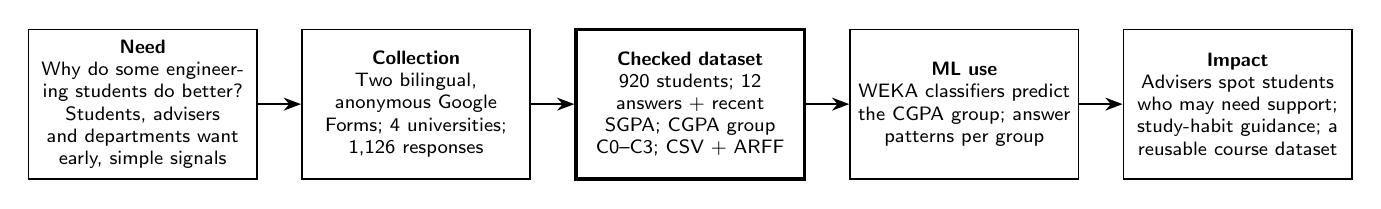
\begin{tikzpicture}[node distance=5.5mm]
\node[box] (a1) {\textbf{Need}\\ Why do some engineering students do better? Students, advisers and departments want early, simple signals};
\node[box, right=of a1] (a2) {\textbf{Collection}\\ Two bilingual, anonymous Google Forms; 4 universities; 1,126 responses};
\node[box, right=of a2, line width=1.2pt] (a3) {\textbf{Checked dataset}\\ 920 students; 12 answers + recent SGPA; CGPA group C0--C3; CSV + ARFF};
\node[box, right=of a3] (a4) {\textbf{ML use}\\ WEKA classifiers predict the CGPA group; answer patterns per group};
\node[box, right=of a4] (a5) {\textbf{Impact}\\ Advisers spot students who may need support; study-habit guidance; a reusable course dataset};
\draw[arr] (a1) -- (a2); \draw[arr] (a2) -- (a3); \draw[arr] (a3) -- (a4); \draw[arr] (a4) -- (a5);
\end{tikzpicture}
\end{center}
\vspace{-3mm}
{\small\itshape Figure 1(a). Practical application of the dataset. Intended users: academic advisers, department heads and students. Practical outcome: simple, explainable signals about which students may need academic support.}

\vspace{2mm}
{\sffamily\bfseries (b) Technical pipeline of the ML method using the dataset}

\begin{center}
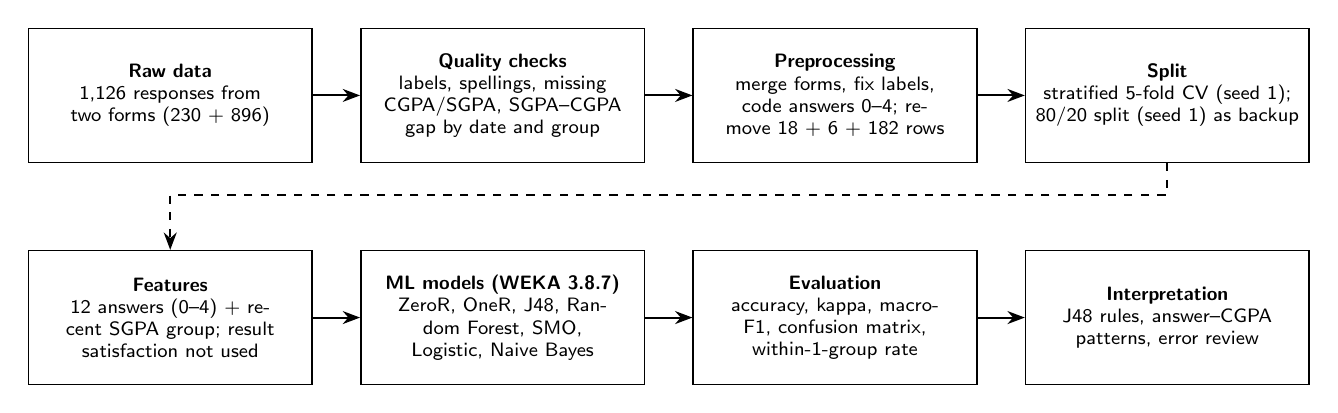
\begin{tikzpicture}[node distance=6mm]
\node[wbox] (b1) {\textbf{Raw data}\\ 1,126 responses from two forms (230 + 896)};
\node[wbox, right=of b1] (b2) {\textbf{Quality checks}\\ labels, spellings, missing CGPA/SGPA, SGPA--CGPA gap by date and group};
\node[wbox, right=of b2] (b3) {\textbf{Preprocessing}\\ merge forms, fix labels, code answers 0--4; remove 18 + 6 + 182 rows};
\node[wbox, right=of b3] (b4) {\textbf{Split}\\ stratified 5-fold CV (seed 1); 80/20 split (seed 1) as backup};
\node[wbox, below=11mm of b1] (c1) {\textbf{Features}\\ 12 answers (0--4) + recent SGPA group; result satisfaction not used};
\node[wbox, right=of c1] (c2) {\textbf{ML models (WEKA 3.8.7)}\\ ZeroR, OneR, J48, Random Forest, SMO, Logistic, Naive Bayes};
\node[wbox, right=of c2] (c3) {\textbf{Evaluation}\\ accuracy, kappa, macro-F1, confusion matrix, within-1-group rate};
\node[wbox, right=of c3] (c4) {\textbf{Interpretation}\\ J48 rules, answer--CGPA patterns, error review};
\draw[arr] (b1) -- (b2); \draw[arr] (b2) -- (b3); \draw[arr] (b3) -- (b4);
\draw[arr] (c1) -- (c2); \draw[arr] (c2) -- (c3); \draw[arr] (c3) -- (c4);
\draw[arr, dashed] (b4.south) -- ++(0,-4mm) -| (c1.north);
\end{tikzpicture}\\[-1mm]
{\small\itshape $\downarrow$ continue with the second row}
\end{center}
\vspace{-3mm}
{\small\itshape Figure 1(b). Technical pipeline followed in the course project. All cleaning is rule-based and fixed before any model is trained, so no statistic is learned from a test fold. Every row is a different anonymous student, so no student can appear in both a training and a test fold.}

\newpage
% =====================================================================================================
\section{1. Dataset Article Information}
{\small
\begin{tabularx}{\linewidth}{L{42mm}Y}
\hline
\hd{Dataset/report title} & What Shapes Student CGPA? A Bilingual Survey Dataset of Study Habits, Well-being and CGPA Groups of 920 Engineering Students in Bangladesh \\ \hline
\hd{Group and students} & Group [\,\_\_\,]: 2107020 Sheikh Md.\ Galib Mahim; 2107030 Md.\ Eftakar Jaman Arfan; 2107007 Asif Jawad; 2107008 Rakibul Islam; 2107012 Md Enam E Elahi; 2107014 Al Mubtasim Preom \\ \hline
\hd{Affiliation} & Department of CSE, KUET, Khulna-9203, Bangladesh \\ \hline
\hd{Corresponding student} & Sheikh Md.\ Galib Mahim, 2107020, [institutional e-mail] \\ \hline
\hd{Keywords} & educational data mining; engineering students; CGPA; study habits; survey data quality; careless responses; WEKA; ordinal classification \\ \hline
\hd{Dataset version} & v1.0; released 15 September 2026 \\ \hline
\hd{Repository / persistent ID} & GitHub: \url{https://github.com/SheikhGalib/CGPA-does-matter-dataset-ml-lab}; no DOI assigned yet \\ \hline
\hd{License} & CC BY 4.0 (proposed for the anonymised, processed files) \\ \hline
\hd{Related article / source} & None (primary data collected by the group) \\ \hline
\end{tabularx}}

% =====================================================================================================
\section{2. Abstract}
We built this dataset to see which everyday student habits and circumstances go together with better or worse cumulative grades (CGPA) among engineering students in Bangladesh. We collected it with two anonymous, bilingual (English and Bangla) Google Forms. The first form reached students of BUET, BRAC University and CUET (230 responses, 22 August to 3 September 2026). The second reached KUET students (896 responses, 31 July to 13 August 2026). Both forms asked the same core questions: department, semester, the SGPA of the last semester, the current CGPA as a range, and fifteen five-option questions about attendance, self-study time, study style, how clear lectures were, sleep, stress, outside commitments, phone distraction, living place, family support, routine, and satisfaction with admission, career path and result. We merged the two forms into one schema, removed the Bangla part of each answer, fixed 110 department spellings, and turned both grade formats into four CGPA groups (C0: below 3.20, C1: 3.20--3.49, C2: 3.50--3.74, C3: 3.75 and above). A data check compared each student's recent SGPA group with their CGPA group. It found one batch of KUET answers, sent on 6--7 August, where the two were often far apart. We removed the 182 answers from that batch whose groups were two or three steps apart. The released version has 920 rows (KUET 690, BUET 104, BRAC 101, CUET 25) with 12 coded answers, the recent SGPA group and the CGPA group, in CSV and WEKA ARFF formats. It also includes the raw exports, a data dictionary, answer codes, the list of removed rows and scripts that rebuild every file. The data can be reused for teaching classification, for studying survey data quality, and for comparing student habits across universities.

% =====================================================================================================
\section{3. Dataset Specifications Table}
{\small
\begin{tabularx}{\linewidth}{|L{40mm}|Y|}
\hline
\rowcolor{hdr}\hd{Item} & \hd{Required information} \\ \hline
\hd{Subject / domain} & Education (higher education, educational data mining) \\ \hline
\hd{Specific subject area} & Self-reported study habits, well-being, support and CGPA groups of undergraduate engineering students in Bangladesh \\ \hline
\hd{Type of data} & Tabular survey data; raw (two Google Forms exports) and processed (cleaned, coded, checked) \\ \hline
\hd{File formats} & CSV (UTF-8), ARFF (WEKA), JSON (summary numbers), Markdown and PDF (documentation), PNG (figures); all open formats \\ \hline
\hd{Unit of observation} & One row = one anonymous form response from one student \\ \hline
\hd{Data collection / source} & Primary collection through two online questionnaires (Google Forms), shared in university student groups \\ \hline
\hd{Instrument / software} & Google Forms (bilingual questions, single-choice answers); Python 3.14.5 (pandas 3.0.5, NumPy 2.5.2, SciPy 1.18.1, matplotlib 3.11.1) for cleaning; WEKA 3.8.7 for modelling \\ \hline
\hd{Data source location} & Bangladesh: KUET (Khulna), BUET (Dhaka), BRAC University (Dhaka), CUET (Chattogram); online, self-completed \\ \hline
\hd{Collection period} & 31 July 2026 -- 3 September 2026 (KUET form: 31 Jul -- 13 Aug; multi-university form: 22 Aug -- 3 Sep) \\ \hline
\hd{Dataset size} & Raw: 1,126 responses (22 + 21 columns). Clean: 1,108 rows. Released ML file: 920 rows, 14 attributes (12 coded answers, recent SGPA group, CGPA group); 4 classes; about 32 KB (CSV) \\ \hline
\hd{Target / labels} & \texttt{cgpa\_band}: C0 below 3.20 (182), C1 3.20--3.49 (284), C2 3.50--3.74 (264), C3 3.75 and above (190); self-reported by each student \\ \hline
\hd{Accessibility} & \url{https://github.com/SheikhGalib/CGPA-does-matter-dataset-ml-lab}, folders \texttt{raw-data/} and \texttt{cleaned-dataset/ours/final/} \\ \hline
\hd{License / reuse terms} & CC BY 4.0 (proposed). Anonymous data; no names, roll numbers or e-mail addresses. Do not try to re-identify respondents \\ \hline
\end{tabularx}}

% =====================================================================================================
\section{4. Value of the Data}
\begin{itemize}
\item \textbf{Why it is valuable.} It is a real, recent sample of 1,126 engineering students from four Bangladeshi universities. It links everyday habits (attendance, study time, sleep, stress, phone use, outside work) with CGPA groups, and every cleaning and removal step is documented and can be reproduced.
\item \textbf{Who can reuse it.} Machine learning and data mining courses (a small, balanced four-class problem that runs in WEKA), education researchers, student-welfare offices and academic advisers.
\item \textbf{What tasks it supports.} Multi-class and ordinal classification of CGPA or SGPA groups; feature association studies; decision-rule mining; clustering of student profiles; and data-quality studies, such as finding careless survey answers by comparing linked questions.
\item \textbf{How it can be extended.} The same questionnaire can be re-run at other universities or in later semesters and added directly, because answers are stored with fixed codes. The per-question tables make it easy to compare with public datasets such as the UCI Student Performance data [4].
\item \textbf{A worked data-quality case.} The dataset shows, with evidence, how one batch of rushed answers can hide real patterns. Accuracy of the same models rose from about 46\% to 55\% after the check (Section 10.7).
\end{itemize}

% =====================================================================================================
\section{5. Background and Practical Motivation}
Engineering programmes in Bangladesh are demanding, and a low CGPA can limit scholarships, higher study and jobs. Teachers and advisers usually learn about a struggling student only after results are published. Students also receive a lot of advice (``attend every class'', ``sleep more'', ``stay off your phone'') without local evidence of how these habits relate to grades in their own programmes.

Most public student-performance datasets come from other countries or other levels of education: Portuguese secondary schools [4], a Portuguese polytechnic's administrative records [5], a Cypriot university survey of 145 students [6], or learning-management-system logs [7]. Recent Bangladeshi work looks at school-level SSC/HSC results or school course grades [2], [3]. We found no open, documented dataset that links study behaviour to CGPA for engineering undergraduates across several Bangladeshi universities.

Our group therefore designed a short, anonymous questionnaire and collected responses at KUET, BUET, BRAC University and CUET. The practical aim, shown in Figure 1(a), is to give advisers and students simple signals: which answers appear more often in the lower or higher CGPA groups, and how well a small set of answers can place a student in a CGPA group. A second aim came from the data itself. While modelling, we noticed that many students' recent SGPA and CGPA were far apart. We traced this to one batch of submissions, so the dataset also records how survey answer quality was checked. We are not trying to prove what causes a high CGPA. The data is observational and self-reported, and we describe it that way throughout.

% =====================================================================================================
\section{6. Data Acquisition / Experimental Design, Materials and Methods}
All data are \textbf{primary data} collected by the group. No external or secondary dataset was merged into the released files.

\subsection{6.1 Data source and sampling strategy}
\textbf{Population.} Undergraduate students of engineering universities in Bangladesh who were enrolled in 2026.

\textbf{Sampling method.} We used convenience sampling with self-selection. Form links were shared in class and department messenger groups and passed on by students. At KUET the form was shared across departments and semesters. Semester-7 students (the group's own cohort) responded most, which gives 675 of the 872 KUET rows that have a real SGPA. The multi-university form was shared through contacts at BUET, BRAC University and CUET.

\textbf{Inclusion criteria.} The respondent is a current undergraduate student and submitted the form.

\textbf{Exclusion criteria.} We removed a response when (i) there was no usable CGPA answer (18 rows); (ii) there was no real recent-SGPA answer (6 rows); or (iii) it came from the 6--7 August KUET semester-7 batch and its SGPA and CGPA groups were two or three steps apart (182 rows). Section 8 gives the reason for each rule.

\textbf{Sample size.} No target size was fixed in advance. We collected as many responses as possible within the course timeline. With four almost balanced classes and 13 inputs, 920 rows give about 230 students per class, enough for 5-fold cross-validation with 184 test students in each fold.

\subsection{6.2 Collection setting, period and location}
Students filled in the forms online, on their own phones or computers, at a time they chose. No incentive was offered. Table~\ref{tab:sources} and Figure~\ref{fig:timeline} show the two collection windows. The KUET form ran from 31 July to 13 August 2026. Most of its answers arrived on 5--7 August (99, 326 and 132 per day) and 9--10 August (100 and 160). The multi-university form ran from 22 August to 3 September 2026. The group members listed on Page 1 designed the forms, shared the links and exported the answers.

\begin{table}[!htbp]
\centering\small
\caption{The two source forms and how many rows each contributes at each stage.}
\label{tab:sources}
\begin{tabularx}{\linewidth}{|Y|L{22mm}|L{35mm}|C{9mm}|R{11mm}|R{11mm}|R{11mm}|}
\hline
\rowcolor{hdr}\hd{Form} & \hd{Universities} & \hd{Collection window} & \hd{Cols} & \hd{Raw} & \hd{Clean} & \hd{Final} \\ \hline
\tabinput{tables/sources.tex}
\end{tabularx}
\end{table}

\begin{figure}[!htbp]
\centering
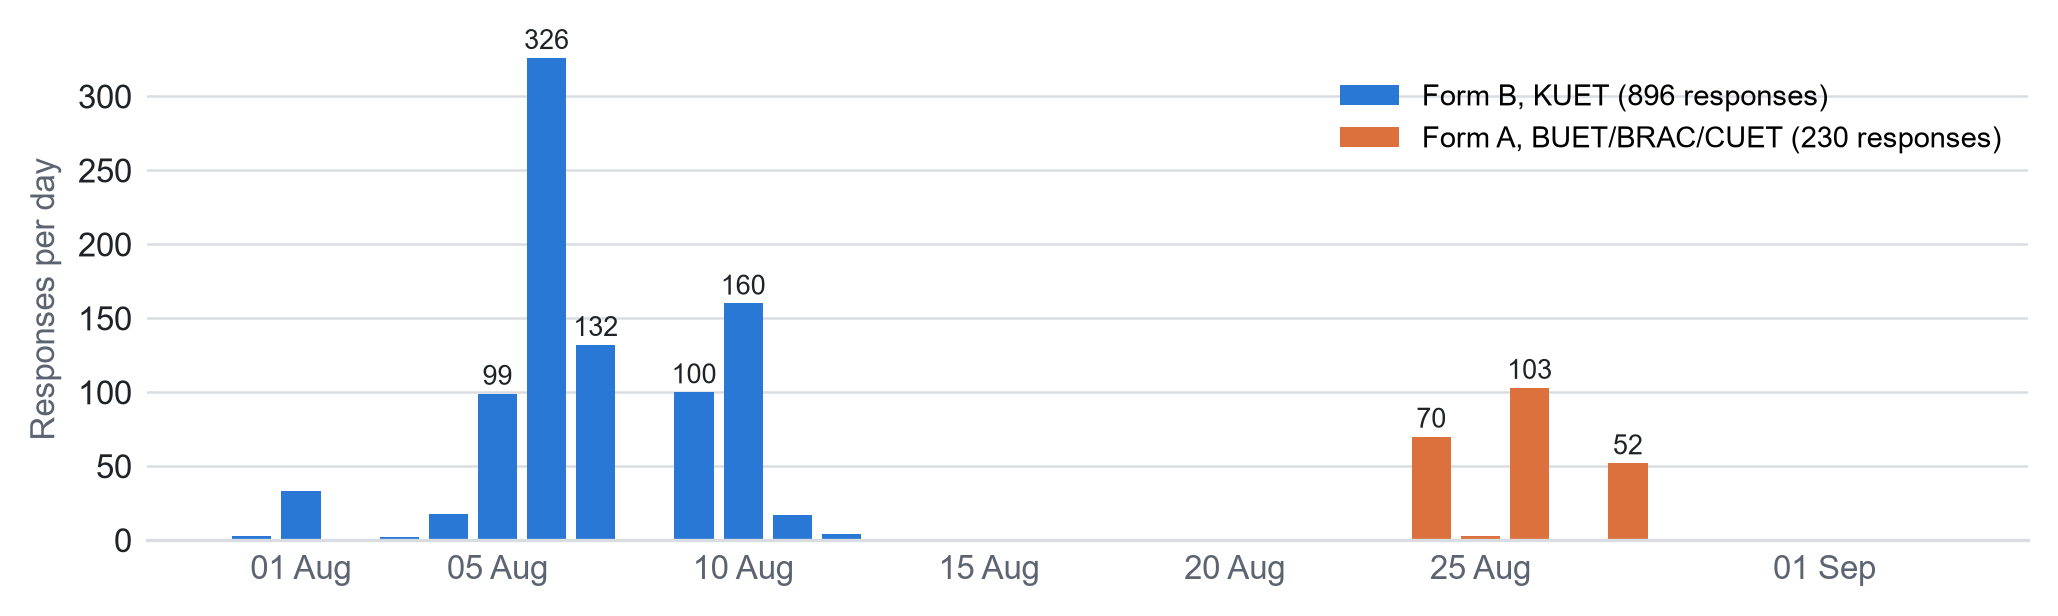
\includegraphics[width=\linewidth]{figures/collection_timeline.png}
\caption{Raw responses received per day. Blue: KUET form (Form B). Orange: multi-university form (Form A). The KUET peak on 6 August is the batch examined in Section 9.}
\label{fig:timeline}
\end{figure}

\subsection{6.3 Instruments, hardware, software and versions}
\begin{itemize}
\item \textbf{Questionnaire.} Two Google Forms written by the group: ``University Student Performance Analysis Form'' (Form A, 22 columns) and ``Student Performance Analysis Form'' (Form B, KUET, 21 columns). Every question is shown in English with a Bangla translation (Figures~\ref{fig:form1}--\ref{fig:form3}). All behaviour questions are single choice with five ordered options. The questions were written for this project and are not copied from a published scale.
\item \textbf{Export.} Google Forms ``Download responses (.csv)'', saved unchanged in \texttt{raw-data/}.
\item \textbf{Cleaning and statistics.} Python 3.14.5 with pandas 3.0.5, NumPy 2.5.2, SciPy 1.18.1 and matplotlib 3.11.1. Scripts: \path{notebooks/02_merged_cleaning_eda_modeling.ipynb} (merge and clean), \path{notebooks/final_weka_results.py} (data check, final files, WEKA runs) and \path{report/build_report_assets.py} (tables and figures in this report).
\item \textbf{Modelling.} WEKA 3.8.7 [8], run from the command line with its bundled Java runtime and also checked in the WEKA Explorer (\texttt{docs/FINAL\_WEKA\_STEPS.md}).
\end{itemize}

\textbf{Screenshots of the Google Form and the response sheet.} Figures~\ref{fig:form1}--\ref{fig:form3} show the actual Google Form the students filled in, and Figure~\ref{fig:rawsheet} shows the Google Sheets response sheet exported from it before any cleaning.

\begin{figure}[!htbp]
\centering
\begin{subfigure}[t]{0.40\linewidth}\centering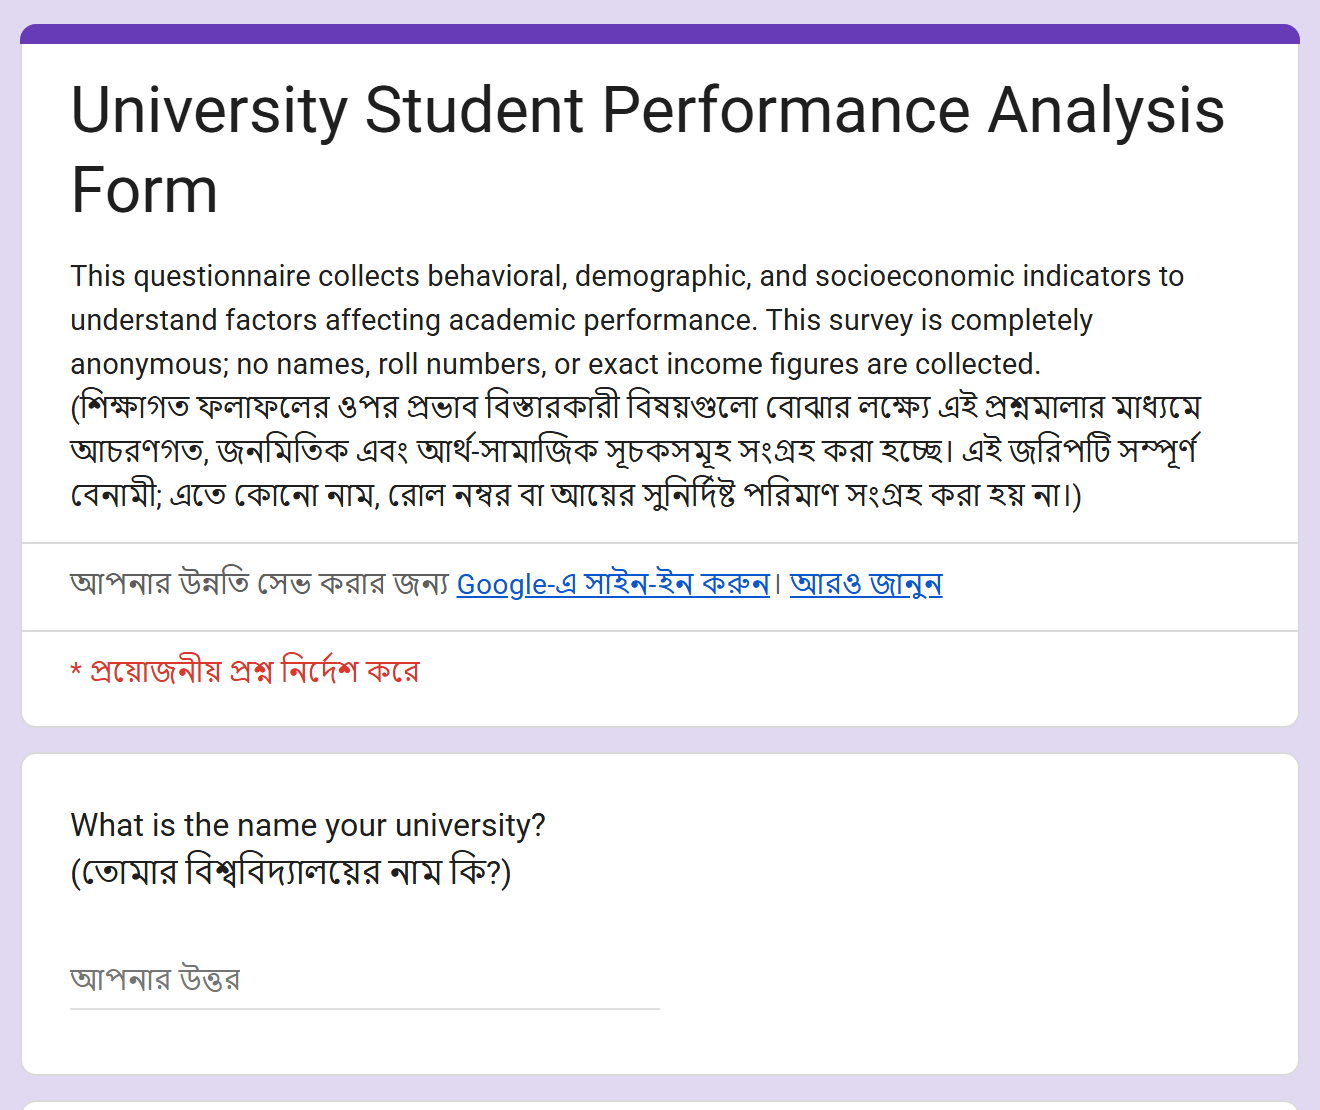
\includegraphics[width=\linewidth]{figures/form/s04_05.png}\caption{Form heading, anonymity statement and first question}\end{subfigure}\hfill
\begin{subfigure}[t]{0.58\linewidth}\centering
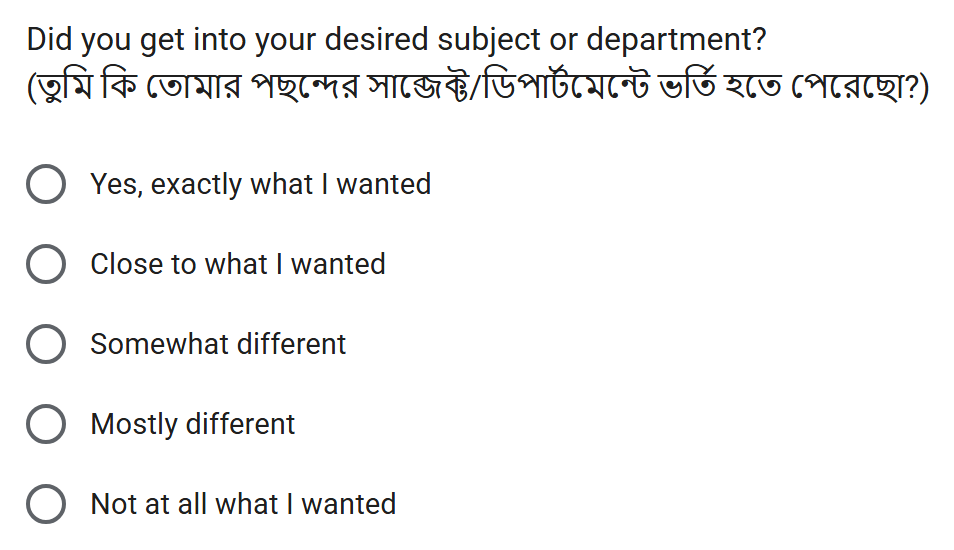
\includegraphics[width=0.49\linewidth]{figures/form/s04_06.png}\hfill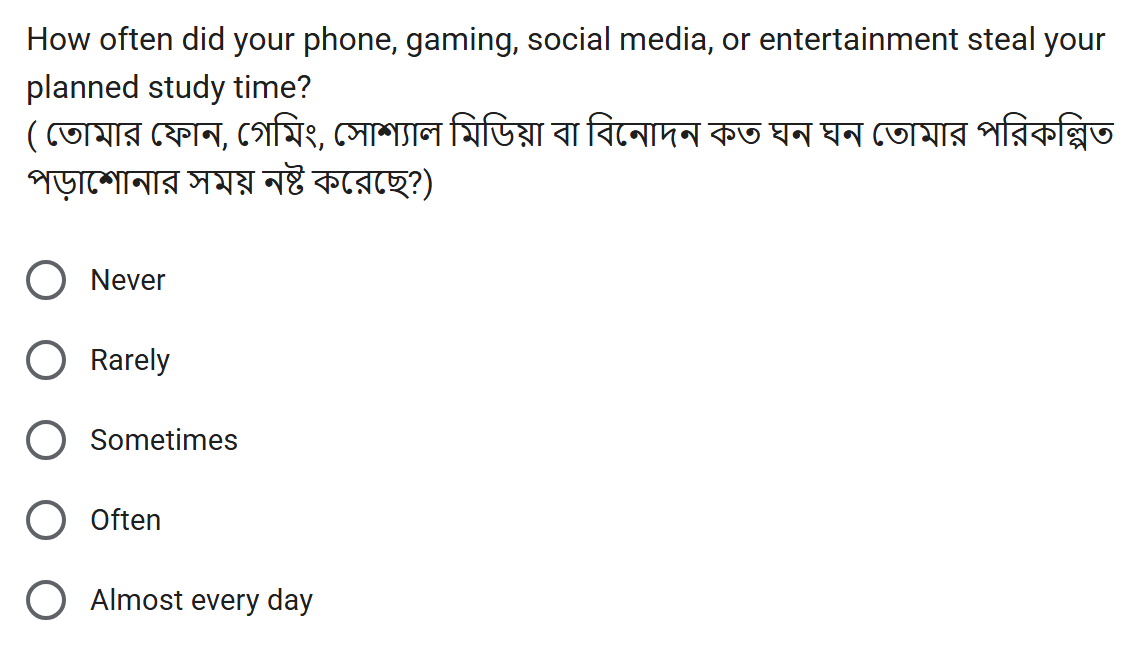
\includegraphics[width=0.49\linewidth]{figures/form/s04_07.png}\\[2mm]
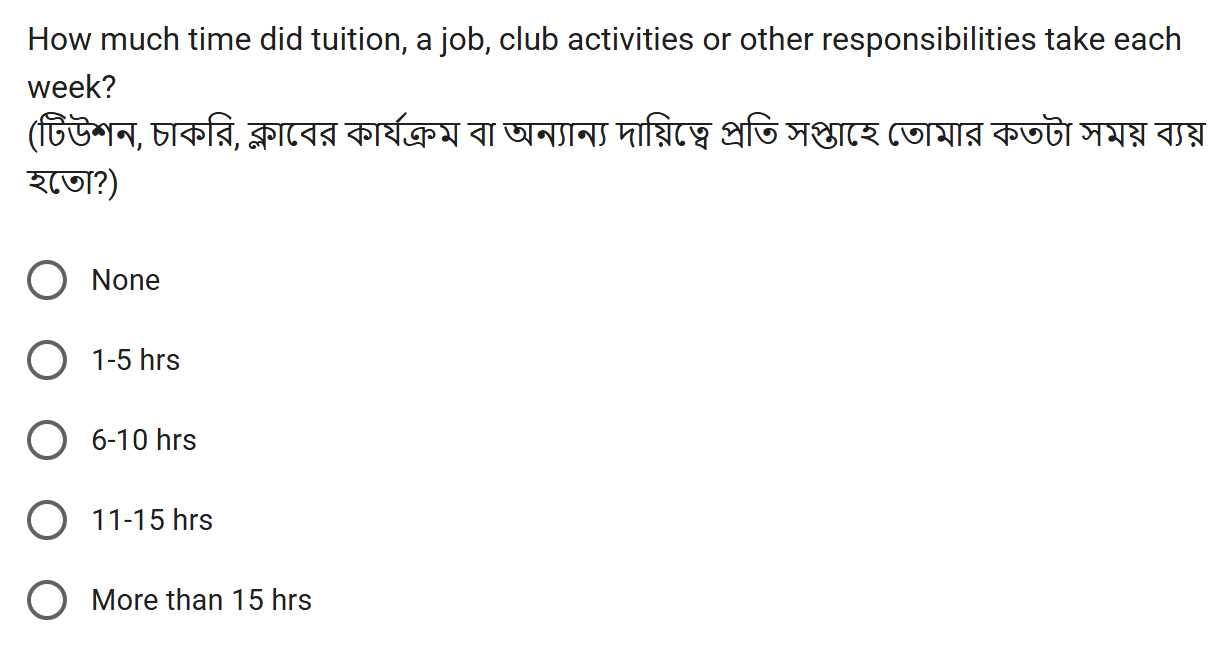
\includegraphics[width=0.49\linewidth]{figures/form/s04_08.png}\hfill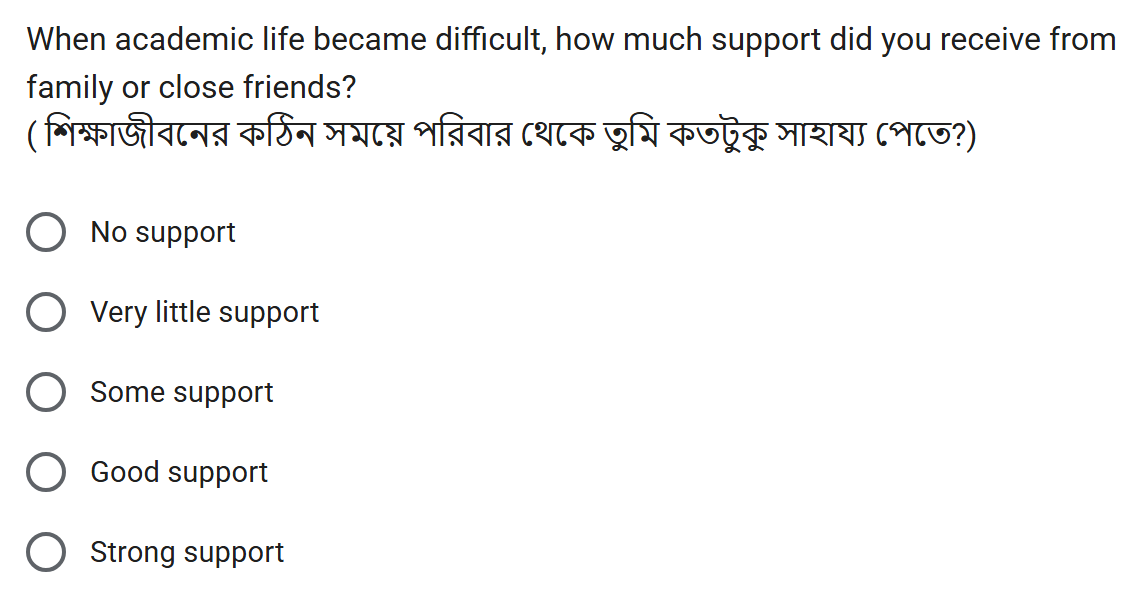
\includegraphics[width=0.49\linewidth]{figures/form/s04_09.png}
\caption{Desired department, phone distraction, outside commitments and family support questions}\end{subfigure}
\caption{Screenshots of the Google Form (University Student Performance Analysis Form). Every question is shown in English and Bangla; answers are single choice.}
\label{fig:form1}
\end{figure}

\begin{figure}[!htbp]
\centering
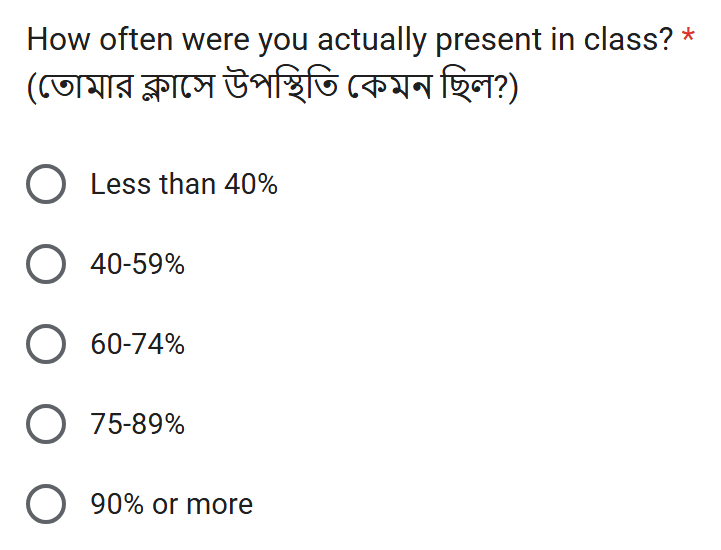
\includegraphics[width=0.40\linewidth]{figures/form/s05_05.png}\hspace{4mm}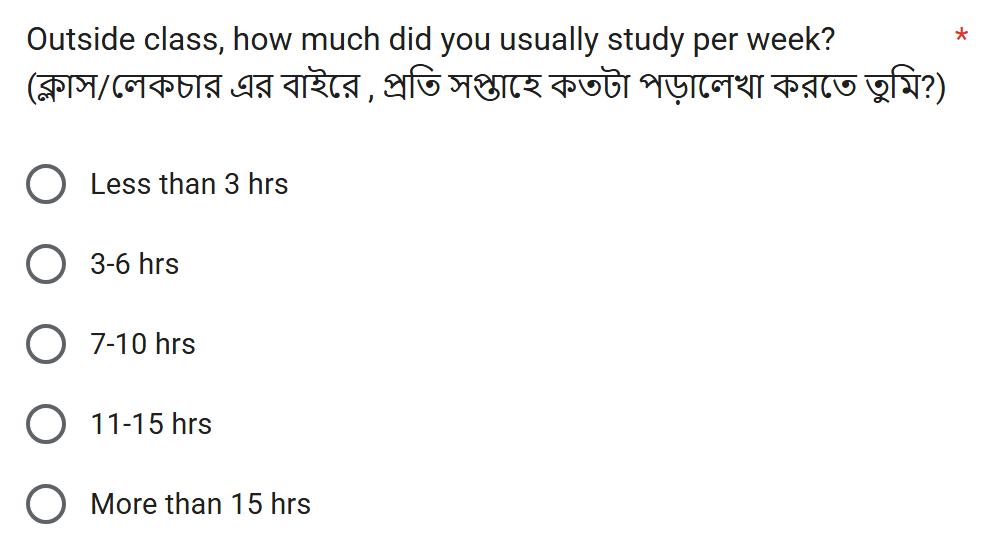
\includegraphics[width=0.50\linewidth]{figures/form/s05_06.png}\\[2mm]
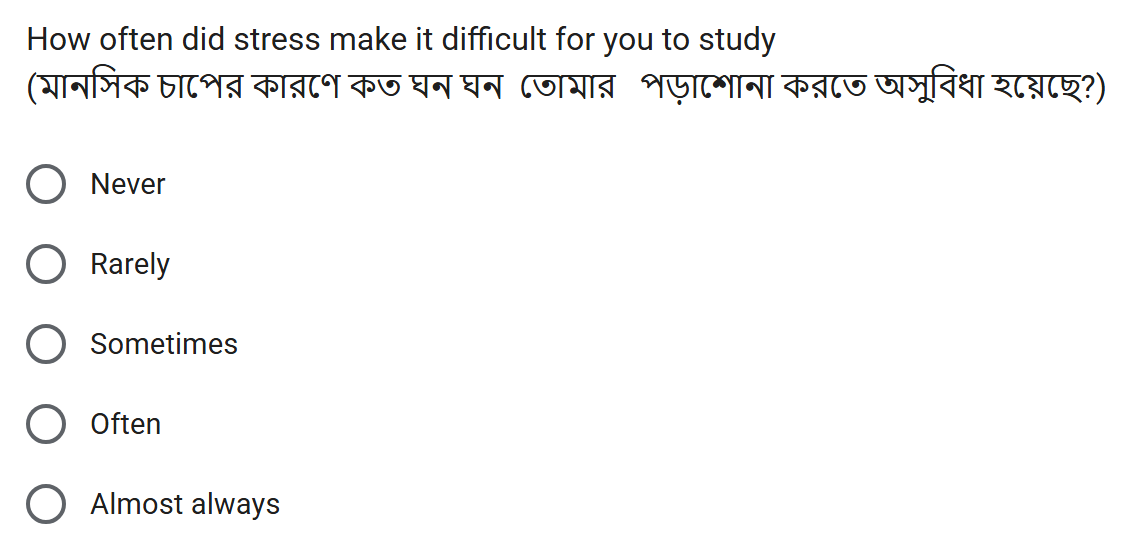
\includegraphics[width=0.52\linewidth]{figures/form/s05_07.png}\hspace{4mm}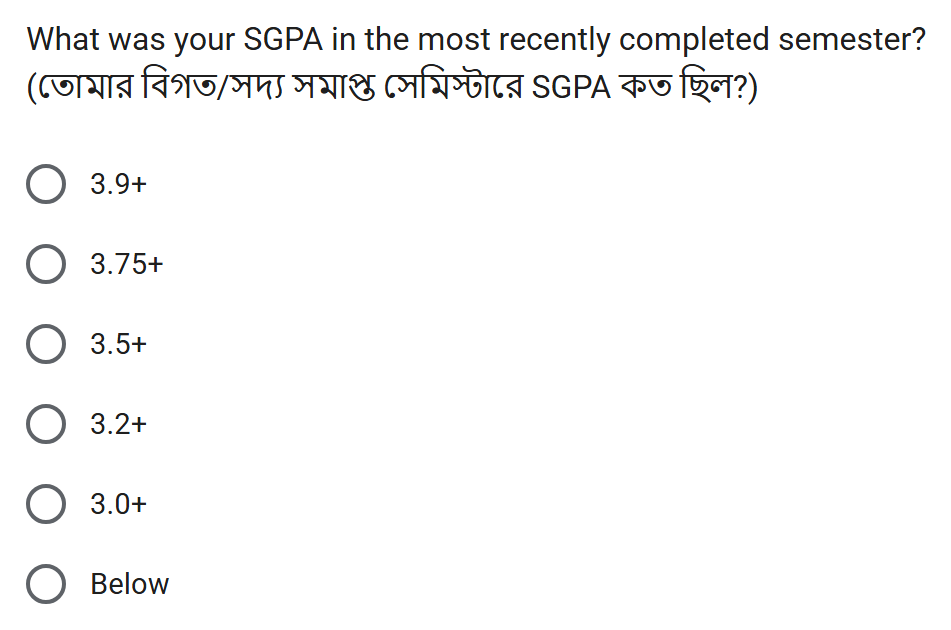
\includegraphics[width=0.40\linewidth]{figures/form/s05_08.png}
\caption{Google Form screenshots: attendance, weekly self-study, stress and recent SGPA questions (the SGPA question shows Form A's six grade ranges).}
\label{fig:form2}
\end{figure}

\begin{figure}[!htbp]
\centering
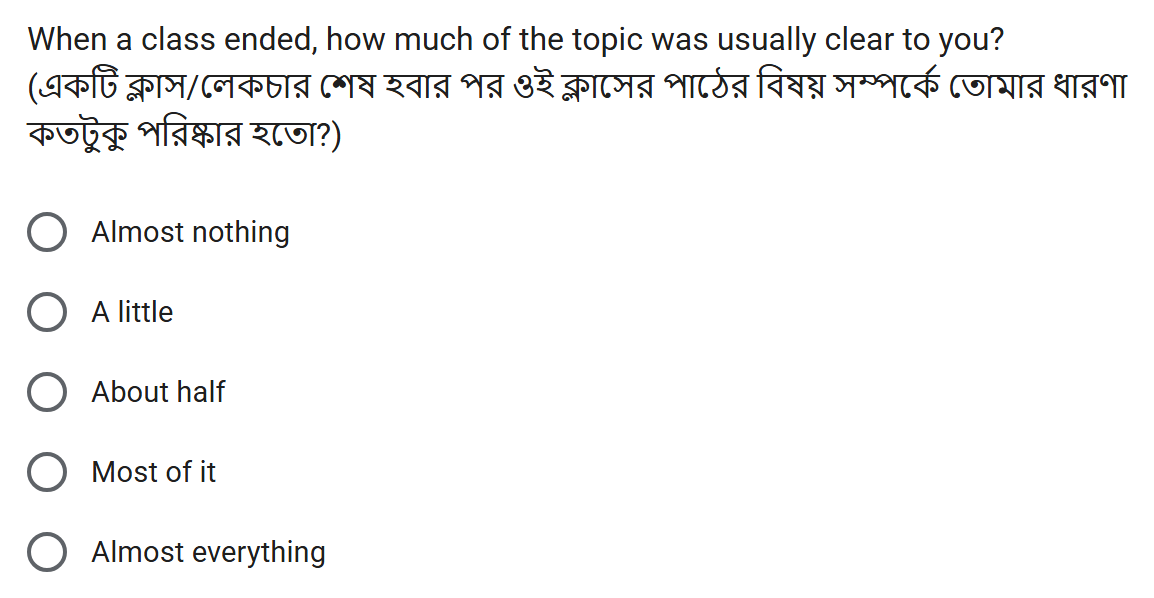
\includegraphics[width=0.32\linewidth]{figures/form/s06_06.png}\hfill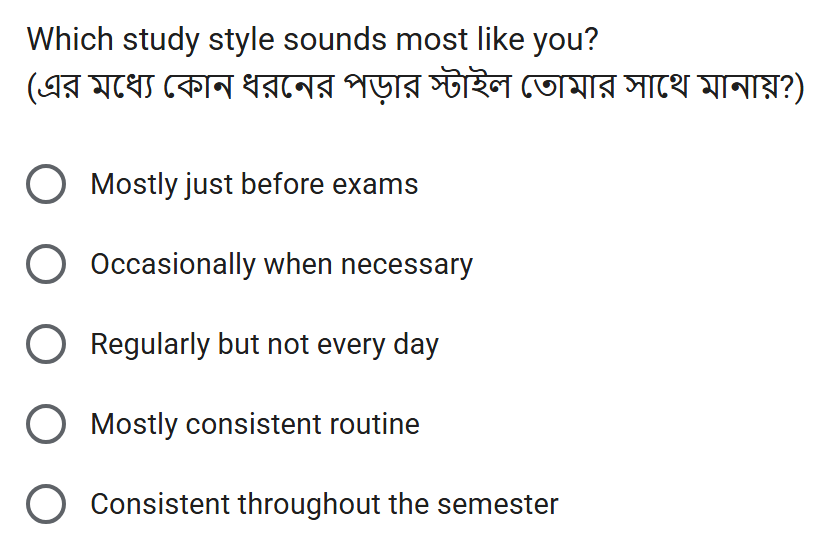
\includegraphics[width=0.32\linewidth]{figures/form/s06_08.png}\hfill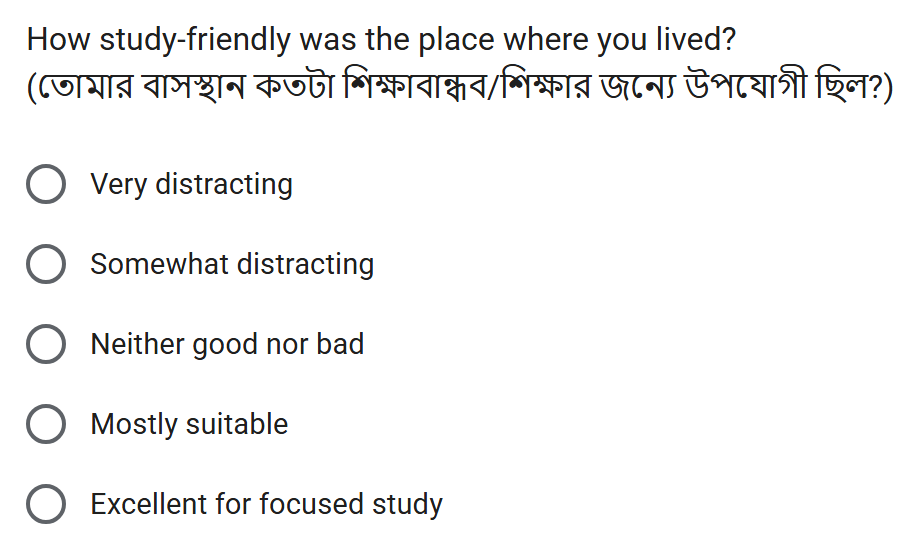
\includegraphics[width=0.32\linewidth]{figures/form/s06_10.png}\\[2mm]
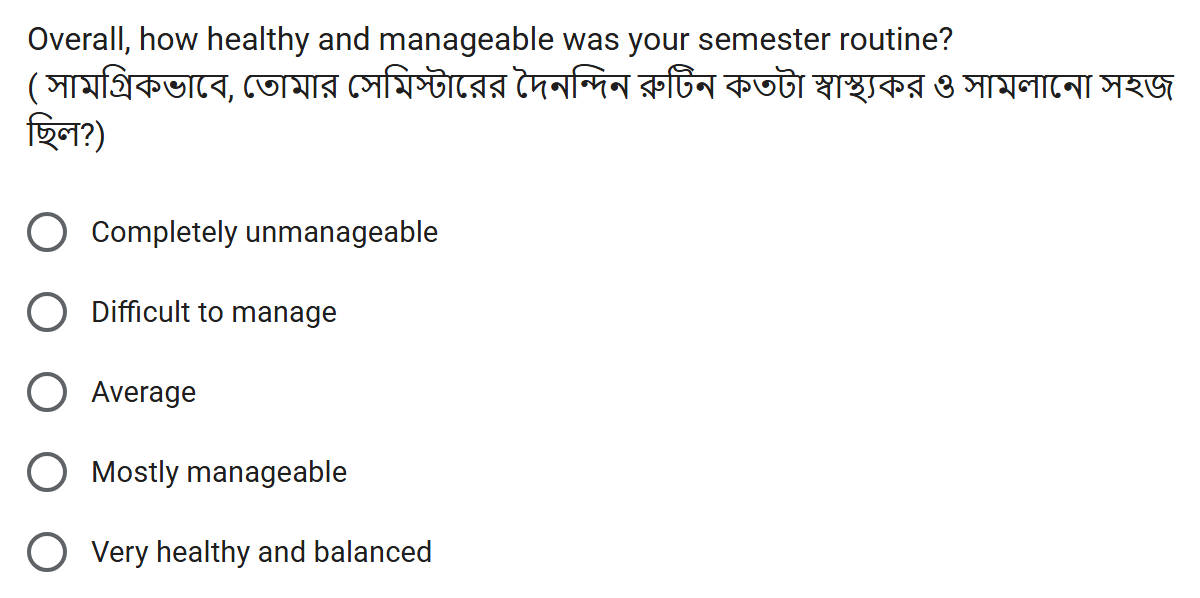
\includegraphics[width=0.32\linewidth]{figures/form/s06_12.png}\hfill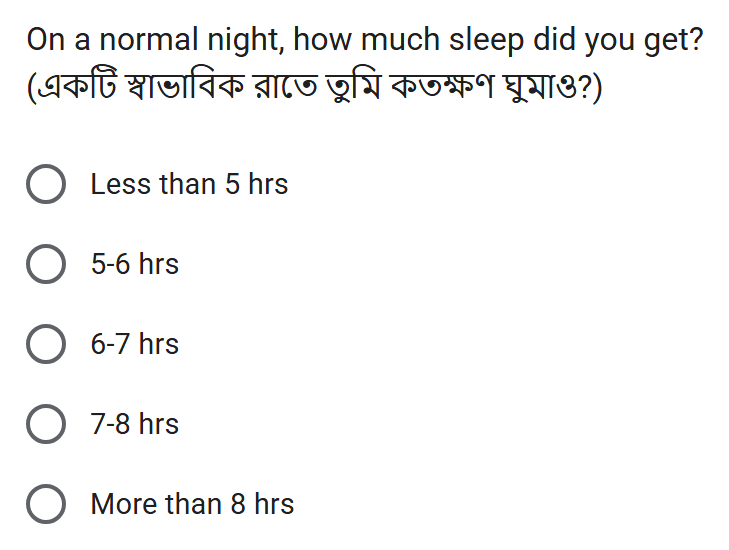
\includegraphics[width=0.32\linewidth]{figures/form/s06_14.png}\hfill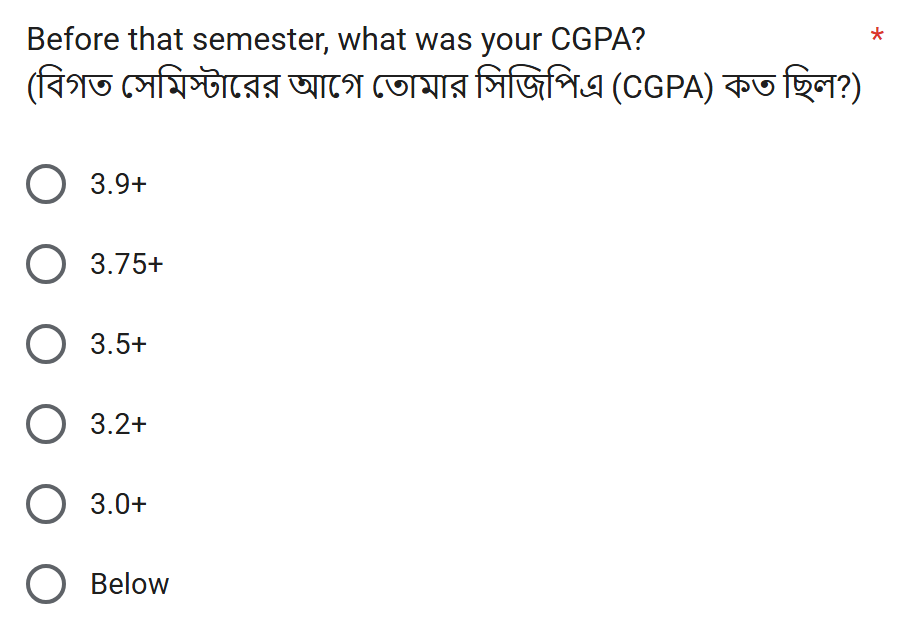
\includegraphics[width=0.32\linewidth]{figures/form/s06_16.png}
\caption{Google Form screenshots: topic clarity, study style, living place, semester routine, sleep and the CGPA question (the class label).}
\label{fig:form3}
\end{figure}

\begin{figure}[!htbp]
\centering
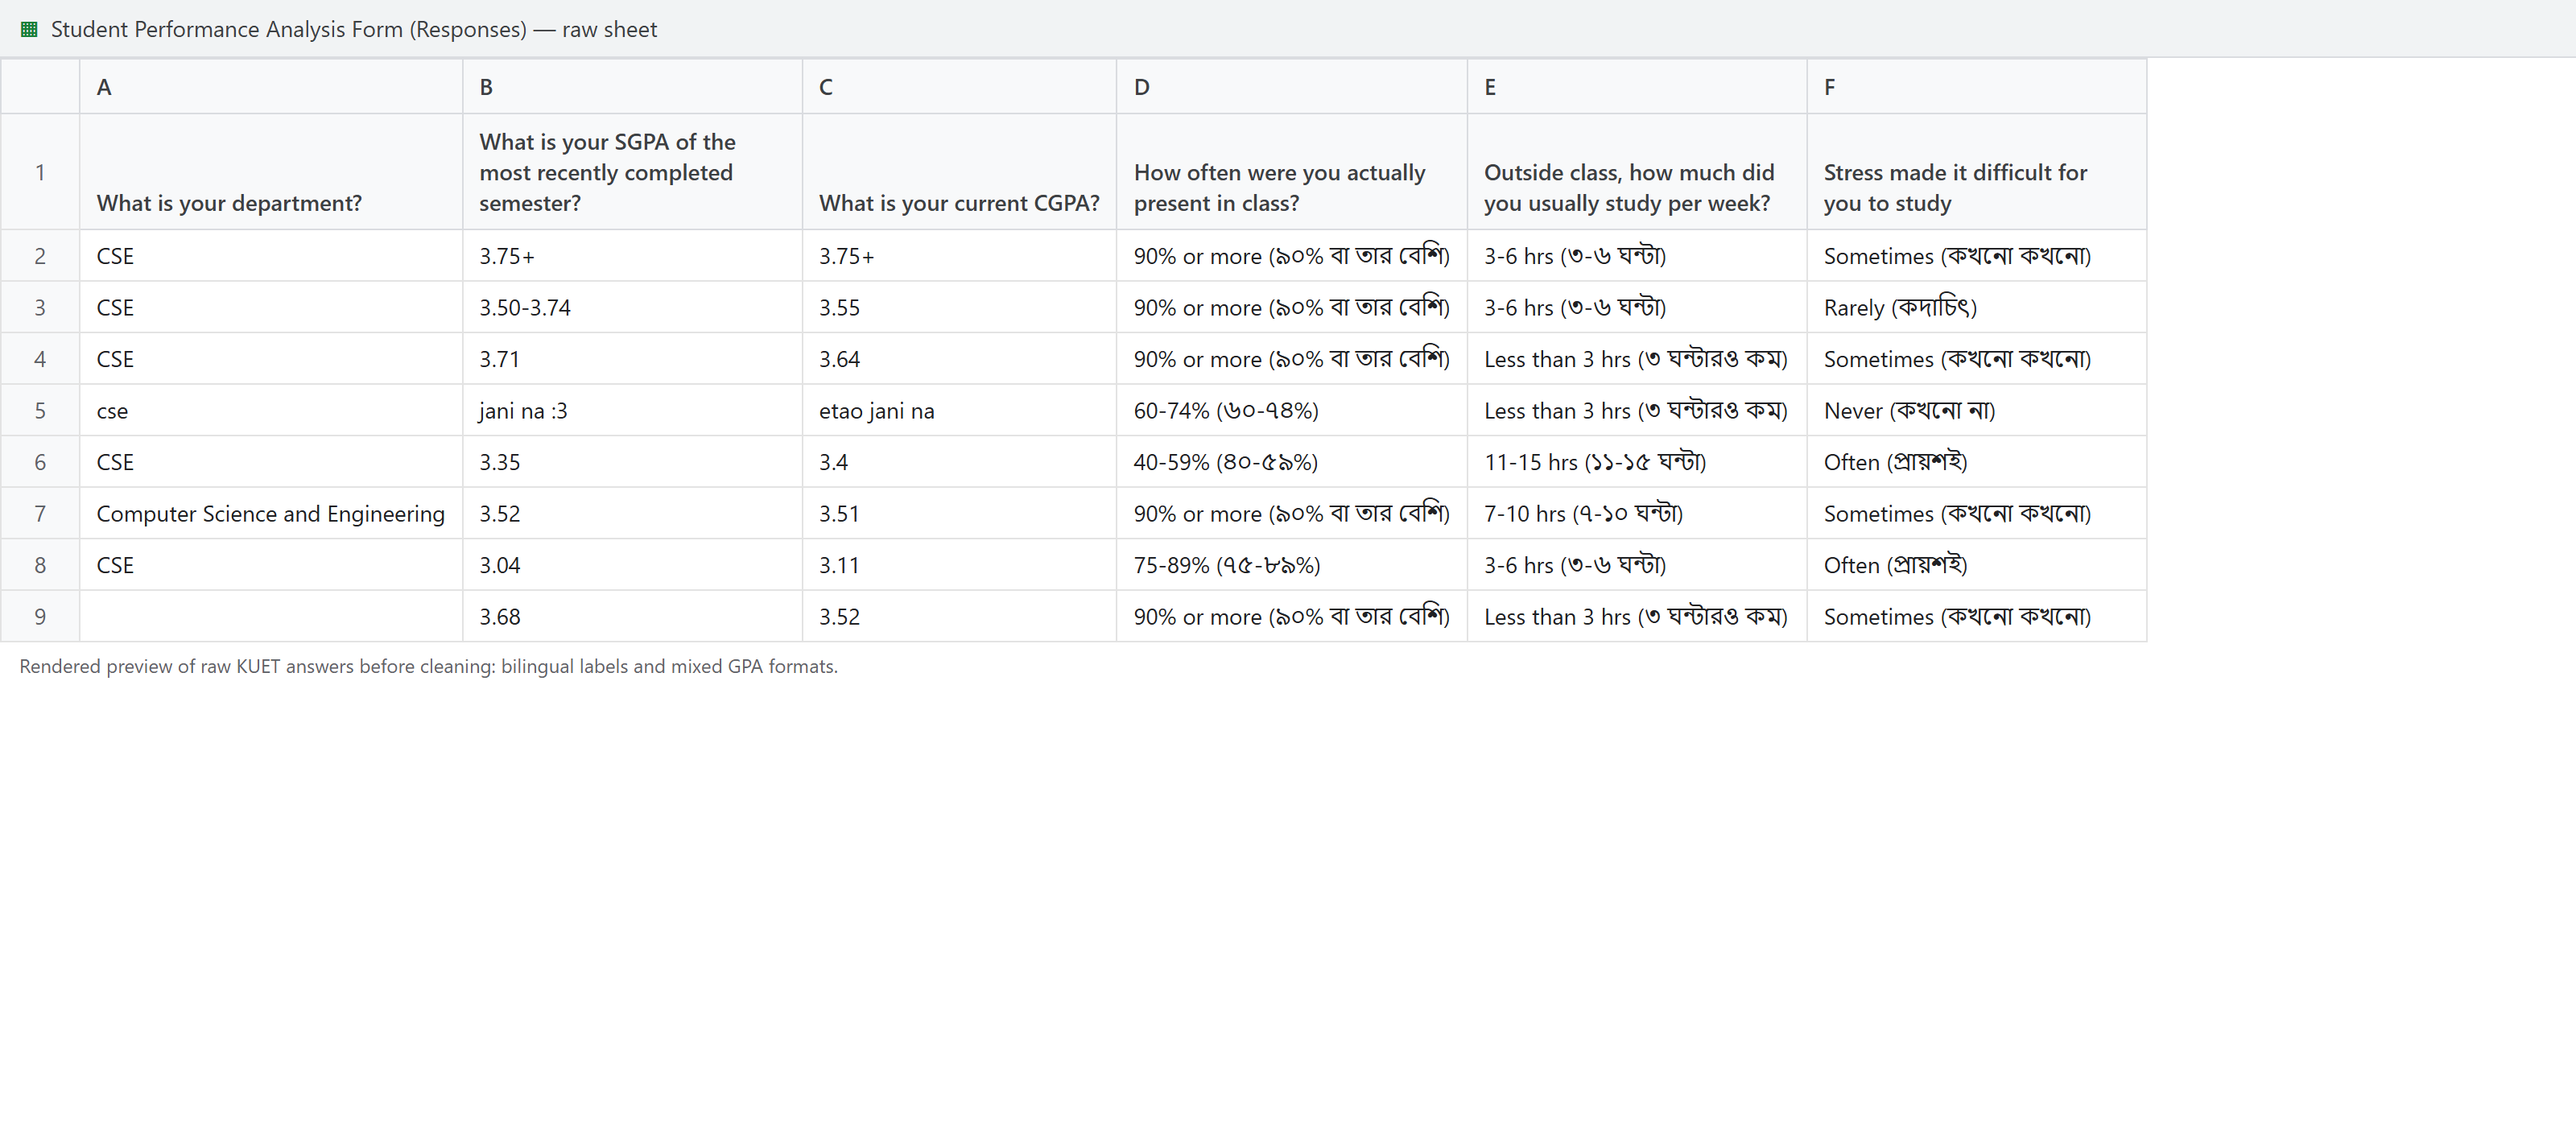
\includegraphics[width=\linewidth,trim=0 540 520 0,clip]{figures/form/s07_00.png}
\caption{The response sheet (KUET form responses) before cleaning. Answers carry Bangla translations, grades appear as ranges or typed numbers, one student typed ``jani na'' (``I don't know''; row removed), and department spellings differ (``CSE'', ``cse'', ``Computer Science and Engineering'').}
\label{fig:rawsheet}
\end{figure}

\subsection{6.4 Variables, measurements and metadata}
Each response records the following. Section 7.2 and Appendix A define every field.
\begin{itemize}
\item \textbf{Context:} university (Form A only; Form B is all KUET), department (free text), current semester.
\item \textbf{Grades (self-reported ranges):} SGPA of the most recently completed semester; CGPA. Form A offered six ranges (Below, 3.0+, 3.2+, 3.5+, 3.75+, 3.9+). Form B offered four ranges or let students type a number.
\item \textbf{Twelve behaviour and situation questions used as model inputs}, each with five ordered answers coded 0 (lowest) to 4 (highest): desired department match, attendance, weekly self-study, study style, topic clarity after class, sleep, stress, outside commitments, phone and social-media distraction, living place, family and friend support, and semester routine.
\item \textbf{Three further questions} (admission satisfaction, career expectation, result satisfaction), kept for description only.
\item \textbf{Metadata:} submission timestamp (used only for the data check, never as a model input) and a \texttt{source\_form} flag.
\end{itemize}
No physical units are involved. Time answers are hour ranges (for example ``6--10 hrs'' per week), and attendance answers are percentage ranges.

\subsection{6.5 Annotation / labeling protocol}
Nobody labelled the data by hand. The class label \texttt{cgpa\_band} is the student's own answer to the CGPA question, mapped to four groups with fixed cut-points: C0 below 3.20, C1 3.20--3.49, C2 3.50--3.74, C3 3.75 and above. Form A's ``Below'' and ``3.0+'' both become C0, and ``3.75+'' and ``3.9+'' both become C3. Typed numbers on Form B (35 students) are put in a group by the same cut-points, and two ``I don't know'' answers (``jani na'') are treated as missing. Four groups were used because Form B never offered finer ranges. The recent SGPA is grouped in the same way and becomes the input \texttt{recent\_sgpa\_band}. Because labels come from the students themselves, there is no inter-rater agreement to report. Section 9 describes how the labels were checked instead.

\subsection{6.6 Provenance, versioning and raw-data preservation}
The two Google Forms exports are stored unchanged in \texttt{raw-data/} and are never edited. Every processed file is rebuilt from them by scripts, so the full history of each change is in code (Section 10.6) and in the cleaning log \texttt{docs/cleaning\_step\_log.csv}. Files are named by stage and row count: \texttt{merged\_*\_clean.csv} (1,108 rows) and \texttt{final\_920.*} (920 rows). The released version is v1.0 (15 September 2026, Git commit \texttt{32ce1ce}). Rows removed by the data check are not deleted from the record. They are listed in \texttt{dropped\_182\_rows.csv} with university, semester, date and gap.

% =====================================================================================================
\section{7. Data Description / Data Records}

\subsection{7.1 Repository / Folder Structure}
{\small
\begin{tabularx}{\linewidth}{|L{62mm}|Y|L{26mm}|}
\hline
\rowcolor{hdr}\hd{Folder / file} & \hd{Contents} & \hd{Raw / processed / metadata} \\ \hline
\texttt{raw-data/} & The two original Google Forms CSV exports (230 and 896 responses) & Raw \\ \hline
\texttt{cleaned-dataset/ours/merged/} & \texttt{merged\_full\_clean.csv} (1,108 rows, every text, code and derived column), \texttt{merged\_primary\_clean.csv}, ARFF versions & Processed \\ \hline
\path{cleaned-dataset/ours/final/final_920.csv}, \path{final_920.arff} & \textbf{Released ML files}: 920 rows, 12 coded answers, recent SGPA group, CGPA group & Processed \\ \hline
\path{cleaned-dataset/ours/final/final_920_with_details.csv} & Same 920 rows plus university, department, semester, form, date, gap and answer text & Processed \\ \hline
\path{cleaned-dataset/ours/final/answer_codes.csv} & Meaning of every code 0--4 for each question & Metadata \\ \hline
\path{cleaned-dataset/ours/final/dropped_182_rows.csv} & The 182 removed answers with university, semester, date, groups and gap & Metadata \\ \hline
\texttt{docs/cleaning\_step\_log.csv}, \texttt{docs/final\_results.json} & Cleaning audit trail; every number reported in the presentation and this report & Metadata \\ \hline
\texttt{docs/weka\_runs/final/} & 67 WEKA output logs (the command is on line 2 of each) & Metadata \\ \hline
\texttt{notebooks/}, \texttt{report/build\_report\_assets.py} & Code that rebuilds all processed files, results, tables and figures & Code \\ \hline
\texttt{AGENTS.md}, \texttt{docs/FINAL\_WEKA\_STEPS.md} & Project README and step-by-step WEKA usage guide & Documentation \\ \hline
\end{tabularx}}

\subsection{7.2 Data Dictionary}
Table~\ref{tab:dict} shows representative fields. Appendix A gives the complete dictionary of all released columns.

\begin{table}[!htbp]
\centering\footnotesize
\caption{Representative fields of \texttt{final\_920.csv} / \texttt{final\_920.arff}.}
\label{tab:dict}
\begin{tabularx}{\linewidth}{|L{30mm}|Y|L{15mm}|L{13mm}|L{42mm}|L{22mm}|}
\hline
\rowcolor{hdr}\hd{Variable / field} & \hd{Meaning} & \hd{Type} & \hd{Unit / range} & \hd{Allowed values / coding} & \hd{Missing-value rule} \\ \hline
\texttt{attendance} & How often the student was present in class & ordinal & 0--4 & 0 Less than 40\%, 1 40--59\%, 2 60--74\%, 3 75--89\%, 4 90\% or more & 2 raw blanks filled with the form's median answer \\ \hline
\texttt{weekly\_study\_time} & Self-study outside class per week & ordinal & 0--4 (hours) & 0 $<$3, 1 3--6, 2 7--10, 3 11--15, 4 $>$15 hrs & median answer of the same form \\ \hline
\texttt{weekly\_\allowbreak responsibilities} & Weekly hours on tuition, job, clubs or other duties & ordinal & 0--4 (hours) & 0 None, 1 1--5, 2 6--10, 3 11--15, 4 $>$15 hrs & blank = ``None'' \\ \hline
\texttt{recent\_sgpa\_band} & SGPA group of the last completed semester & nominal (ordered) & C0--C3 & C0 $<$3.20, C1 3.20--3.49, C2 3.50--3.74, C3 $\geq$3.75 & row removed \\ \hline
\texttt{cgpa\_band} (class) & CGPA group (prediction target) & nominal (ordered) & C0--C3 & same cut-points as SGPA & row removed \\ \hline
\end{tabularx}
\end{table}

\subsection{7.3 Dataset Composition and Descriptive Overview}
This subsection gives the detailed statistics of the released 920 rows: composition by university, class, semester and department (7.3.1); missing values in the raw exports (7.3.2); and the answer distribution of every question with its link to the CGPA groups (7.3.3--7.3.4). Sample raw and processed responses are in Figure~\ref{fig:rawsheet} and Table~\ref{tab:sample}.

\subsubsection{7.3.1 Composition by university, CGPA group, semester and department}
\begin{table}[!htbp]
\centering\small
\caption{Final dataset by university and CGPA group. Semester numbering follows each university's own system: BUET students reported term numbers up to 12, and BRAC students reported trimester numbers.}
\label{tab:unicgpa}
\begin{tabularx}{\linewidth}{|L{16mm}|R{9mm}|R{9mm}|R{9mm}|R{9mm}|R{9mm}|R{9mm}|C{16mm}|Y|}
\hline
\rowcolor{hdr}\hd{University} & \hd{n} & \hd{\%} & \hd{C0} & \hd{C1} & \hd{C2} & \hd{C3} & \hd{Semesters} & \hd{Responses received} \\ \hline
\tabinput{tables/university_cgpa.tex}
\end{tabularx}
\end{table}

The four CGPA groups are close to balanced: the largest group (C1, 30.9\%) is 1.56 times the smallest (C0, 19.8\%). A model that always guesses the largest group is right 30.9\% of the time, and this is the baseline every model must beat. KUET supplies three quarters of the rows. CUET has no student in C0 and only 25 rows, so results for CUET alone are not meaningful. The recent-SGPA groups are C0 171, C1 269, C2 261 and C3 219.

\begin{figure}[!htbp]
\centering
\begin{subfigure}{0.49\linewidth}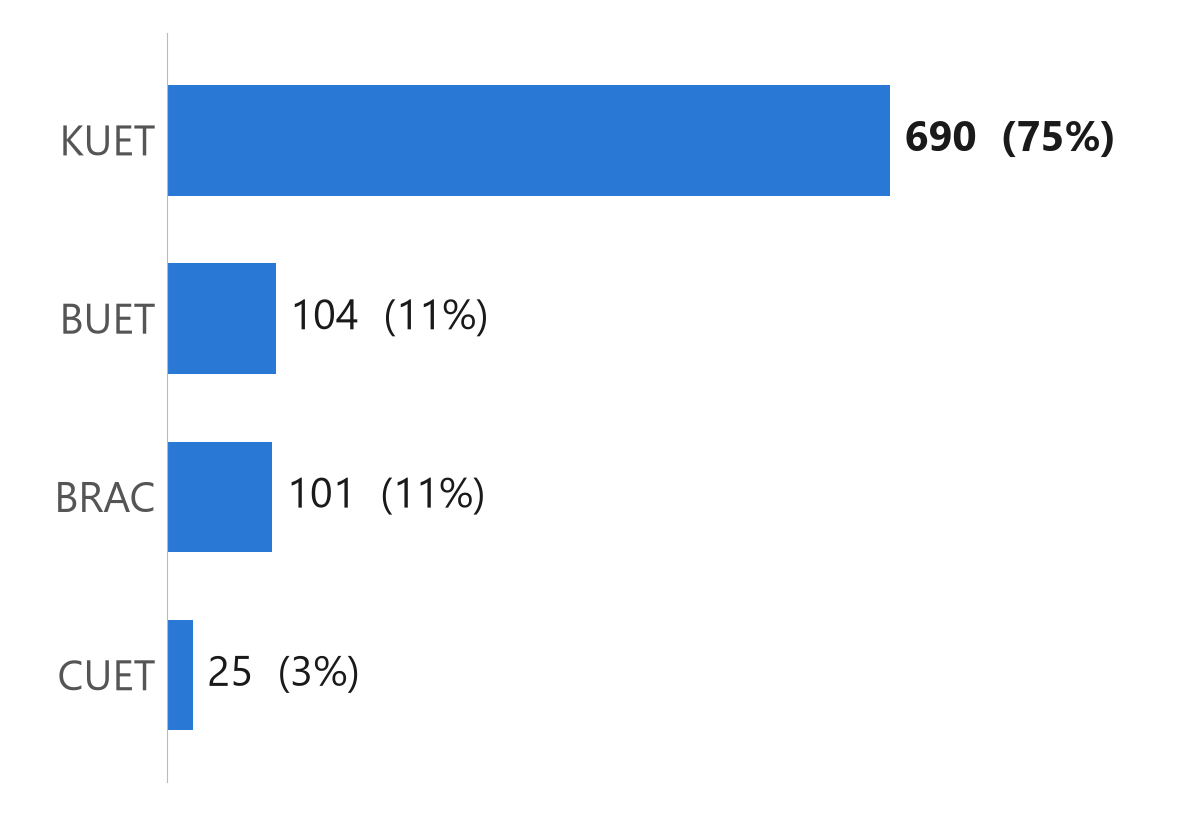
\includegraphics[width=\linewidth]{figures/deck/rc_university.png}\caption{Students per university}\end{subfigure}\hfill
\begin{subfigure}{0.49\linewidth}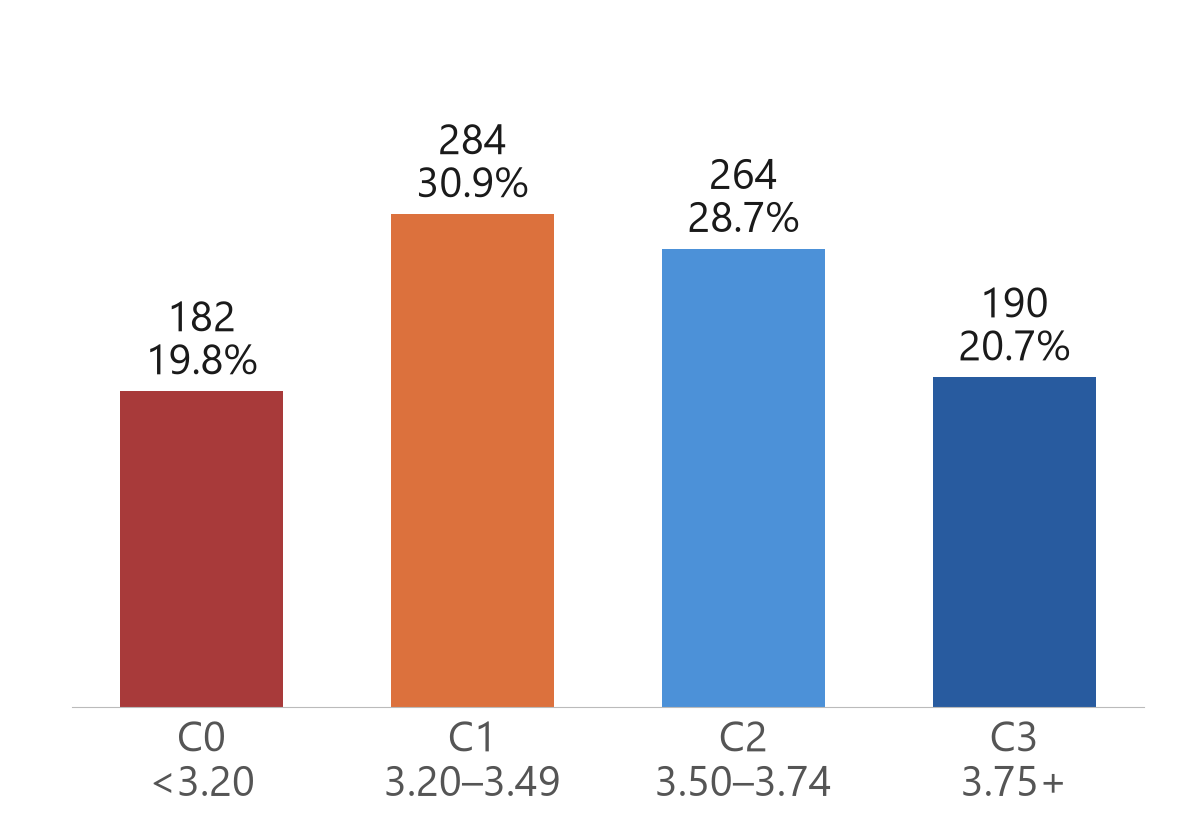
\includegraphics[width=\linewidth]{figures/deck/rc_cgpa.png}\caption{Students per CGPA group}\end{subfigure}
\caption{Composition of the 920 released rows (same charts as the presentation).}
\label{fig:composition}
\end{figure}

\begin{table}[!htbp]
\centering\small
\begin{minipage}[t]{\linewidth}\centering
\captionof{table}{Current semester by university (920 rows).}\label{tab:semester}
\begin{tabular}{|c|r|r|r|r|r|r|}
\hline
\rowcolor{hdr}\hd{Sem} & \hd{KUET} & \hd{BUET} & \hd{BRAC} & \hd{CUET} & \hd{All} & \hd{\%} \\ \hline
\tabinput{tables/semester_university.tex}
\end{tabular}
\end{minipage}\\[5mm]
\begin{minipage}[t]{\linewidth}\centering
\captionof{table}{Department after name cleaning (24 values; 920 rows).}\label{tab:dept}
\begin{tabular}{|l|r|r|l|r|r|}
\hline
\rowcolor{hdr}\hd{Dept.} & \hd{n} & \hd{\%} & \hd{Dept.} & \hd{n} & \hd{\%} \\ \hline
\tabinput{tables/departments.tex}
\end{tabular}
\end{minipage}
\end{table}

\subsubsection{7.3.2 Missing values in the raw exports}
Table~\ref{tab:missing} counts blank answers per question before cleaning. Form A made most questions compulsory, so only its department box has blanks. Its separate ``if not listed'' box is blank in 174 rows by design. On Form B, grades and department have the most blanks; every behaviour question is blank in fewer than 1.6\% of rows. Form B's e-mail column is empty in all 896 rows and was dropped.

\begin{table}[!htbp]
\centering\small
\caption{Blank answers in the raw exports (Form A: 230 rows; Form B: 896 rows; percentage of all 1,126).}
\label{tab:missing}
\begin{tabular}{|l|r|r|r|r|}
\hline
\rowcolor{hdr}\hd{Field} & \hd{Form A} & \hd{Form B} & \hd{Total} & \hd{\% of 1,126} \\ \hline
\tabinput{tables/raw_missing.tex}
\end{tabular}
\end{table}

\subsubsection{7.3.3 Answer distribution of every question}
Figure~\ref{fig:answers} shows how the 920 students answered each of the 12 questions used as model inputs. Figure~\ref{fig:extra} shows the three questions kept for description only. Table~\ref{tab:qsummary} summarises every question in one line.

\begin{figure}[!htbp]
\centering
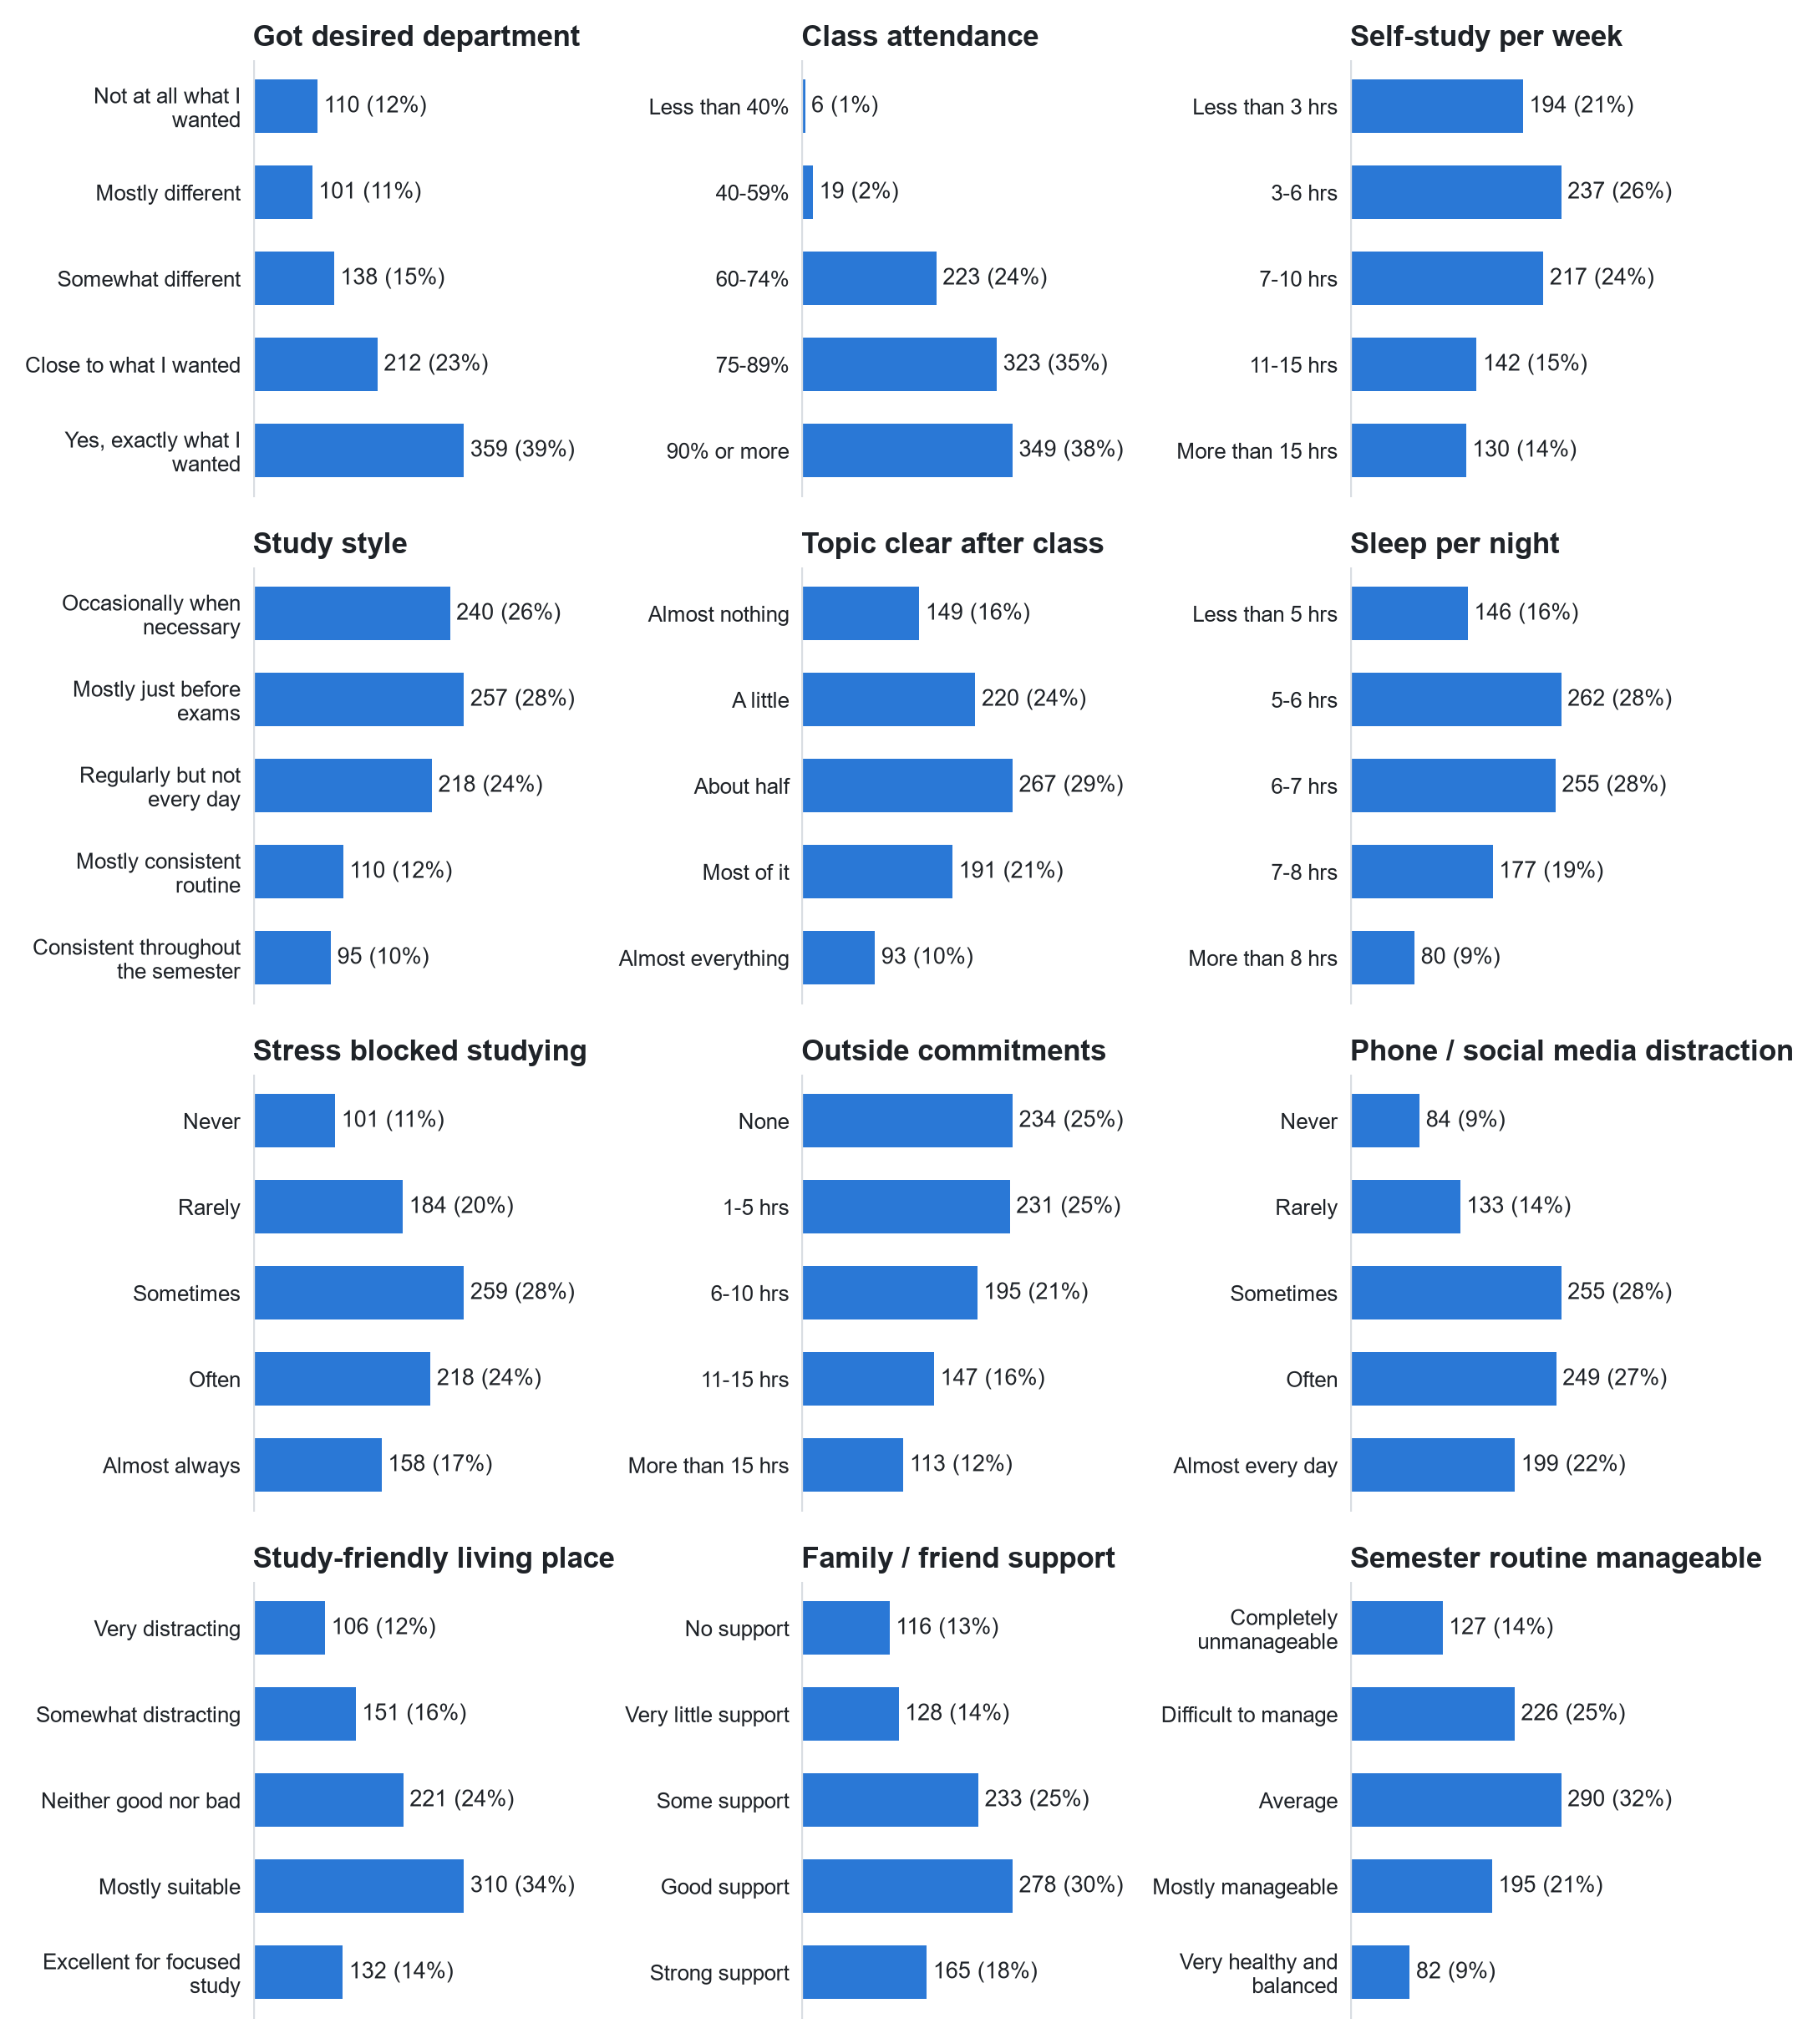
\includegraphics[width=\linewidth]{figures/answers_12_features.png}
\caption{Answers to the 12 model-input questions (n and share of 920 students). Most students attend 75\% of classes or more (73.0\%), 44.3\% sleep less than 6 hours, and 48.7\% say their phone often or almost every day takes study time.}
\label{fig:answers}
\end{figure}

\begin{figure}[!htbp]
\centering
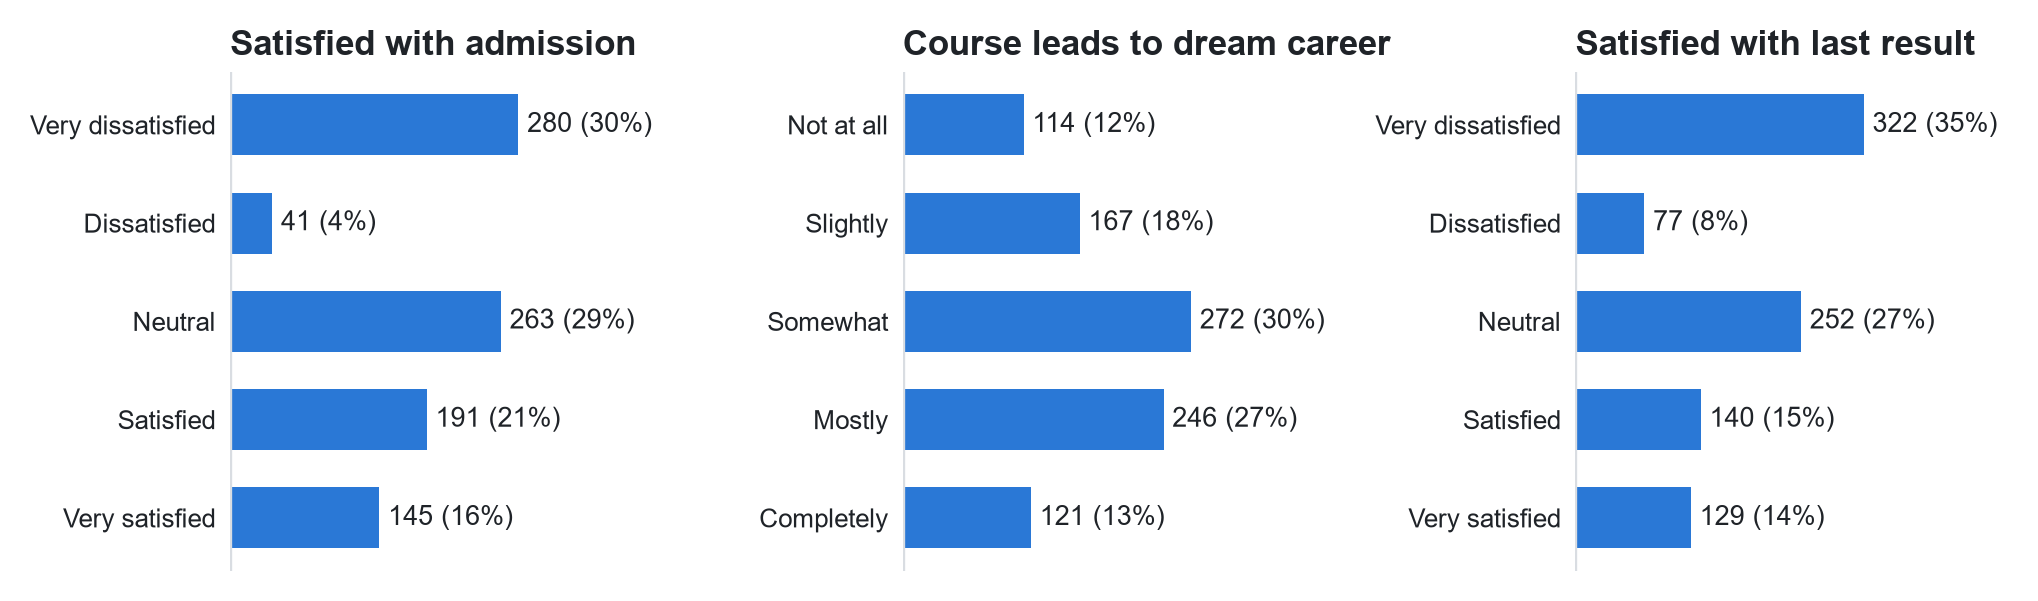
\includegraphics[width=\linewidth]{figures/answers_3_extra.png}
\caption{The three questions kept for description only. Result satisfaction is not used as a model input, because it depends on each student's own expectations. The high share of ``Very dissatisfied'' answers comes mainly from the KUET form (Section 12).}
\label{fig:extra}
\end{figure}

\begin{table}[!htbp]
\centering\scriptsize
\caption{Summary of every question on the 920 rows. Median and mean use the codes 0--4. $\rho$ is the Spearman rank correlation with the CGPA group and with the recent SGPA group. ``Reliable'' means the CGPA correlation stays significant after Benjamini--Hochberg correction for 12 tests ($q<0.05$) [15]. ``Max shift'' is the largest change, in percentage points, of any answer share between the 1,102 rows before the data check and the final 920.}
\label{tab:qsummary}
\begin{tabularx}{\linewidth}{|L{27mm}|Y|Y|R{7mm}|R{6mm}|R{9mm}|R{9mm}|L{11mm}|R{8mm}|}
\hline
\rowcolor{hdr}\hd{Question} & \hd{Most common answer} & \hd{Median answer} & \hd{Mean} & \hd{SD} & \hd{$\rho$ CGPA} & \hd{$\rho$ SGPA} & \hd{Reliable} & \hd{Max shift} \\ \hline
\tabinput{tables/questions_summary.tex}
\end{tabularx}
\end{table}

Only three questions have a reliable link with the CGPA group, and all three links are weak: getting the desired department ($\rho=+0.134$), class attendance ($+0.093$) and outside commitments ($-0.086$). No answer share changed by more than a few percentage points because of the data check, so removing the 182 rows did not reshape the answer distributions.

\subsubsection{7.3.4 Detailed answer statistics per question}
Table~\ref{tab:qdetail} lists every answer option with its code, count and share, and, for the students who chose it, the percentage in each CGPA group (each row of C0--C3 adds up to 100\%). Figures~\ref{fig:mix1} and \ref{fig:mix2} show the same CGPA mix as charts, matching slides 29--40 of the presentation.

{\footnotesize
\setlength{\tabcolsep}{4pt}
\begin{longtable}{|C{8mm}|L{62mm}|R{11mm}|R{11mm}|R{13mm}|R{13mm}|R{13mm}|R{13mm}|}
\caption{Answer-level statistics for all 15 questions (920 rows). n and \% describe the whole sample. C0--C3 are the percentages of the students choosing that answer who are in each CGPA group.}\label{tab:qdetail}\\
\hline
\rowcolor{hdr}\hd{Code} & \hd{Answer} & \hd{n} & \hd{\%} & \hd{C0 \%} & \hd{C1 \%} & \hd{C2 \%} & \hd{C3 \%} \\ \hline
\endfirsthead
\hline
\rowcolor{hdr}\hd{Code} & \hd{Answer} & \hd{n} & \hd{\%} & \hd{C0 \%} & \hd{C1 \%} & \hd{C2 \%} & \hd{C3 \%} \\ \hline
\endhead
\tabinput{tables/questions_detail.tex}
\end{longtable}}

\begin{figure}[!htbp]
\centering
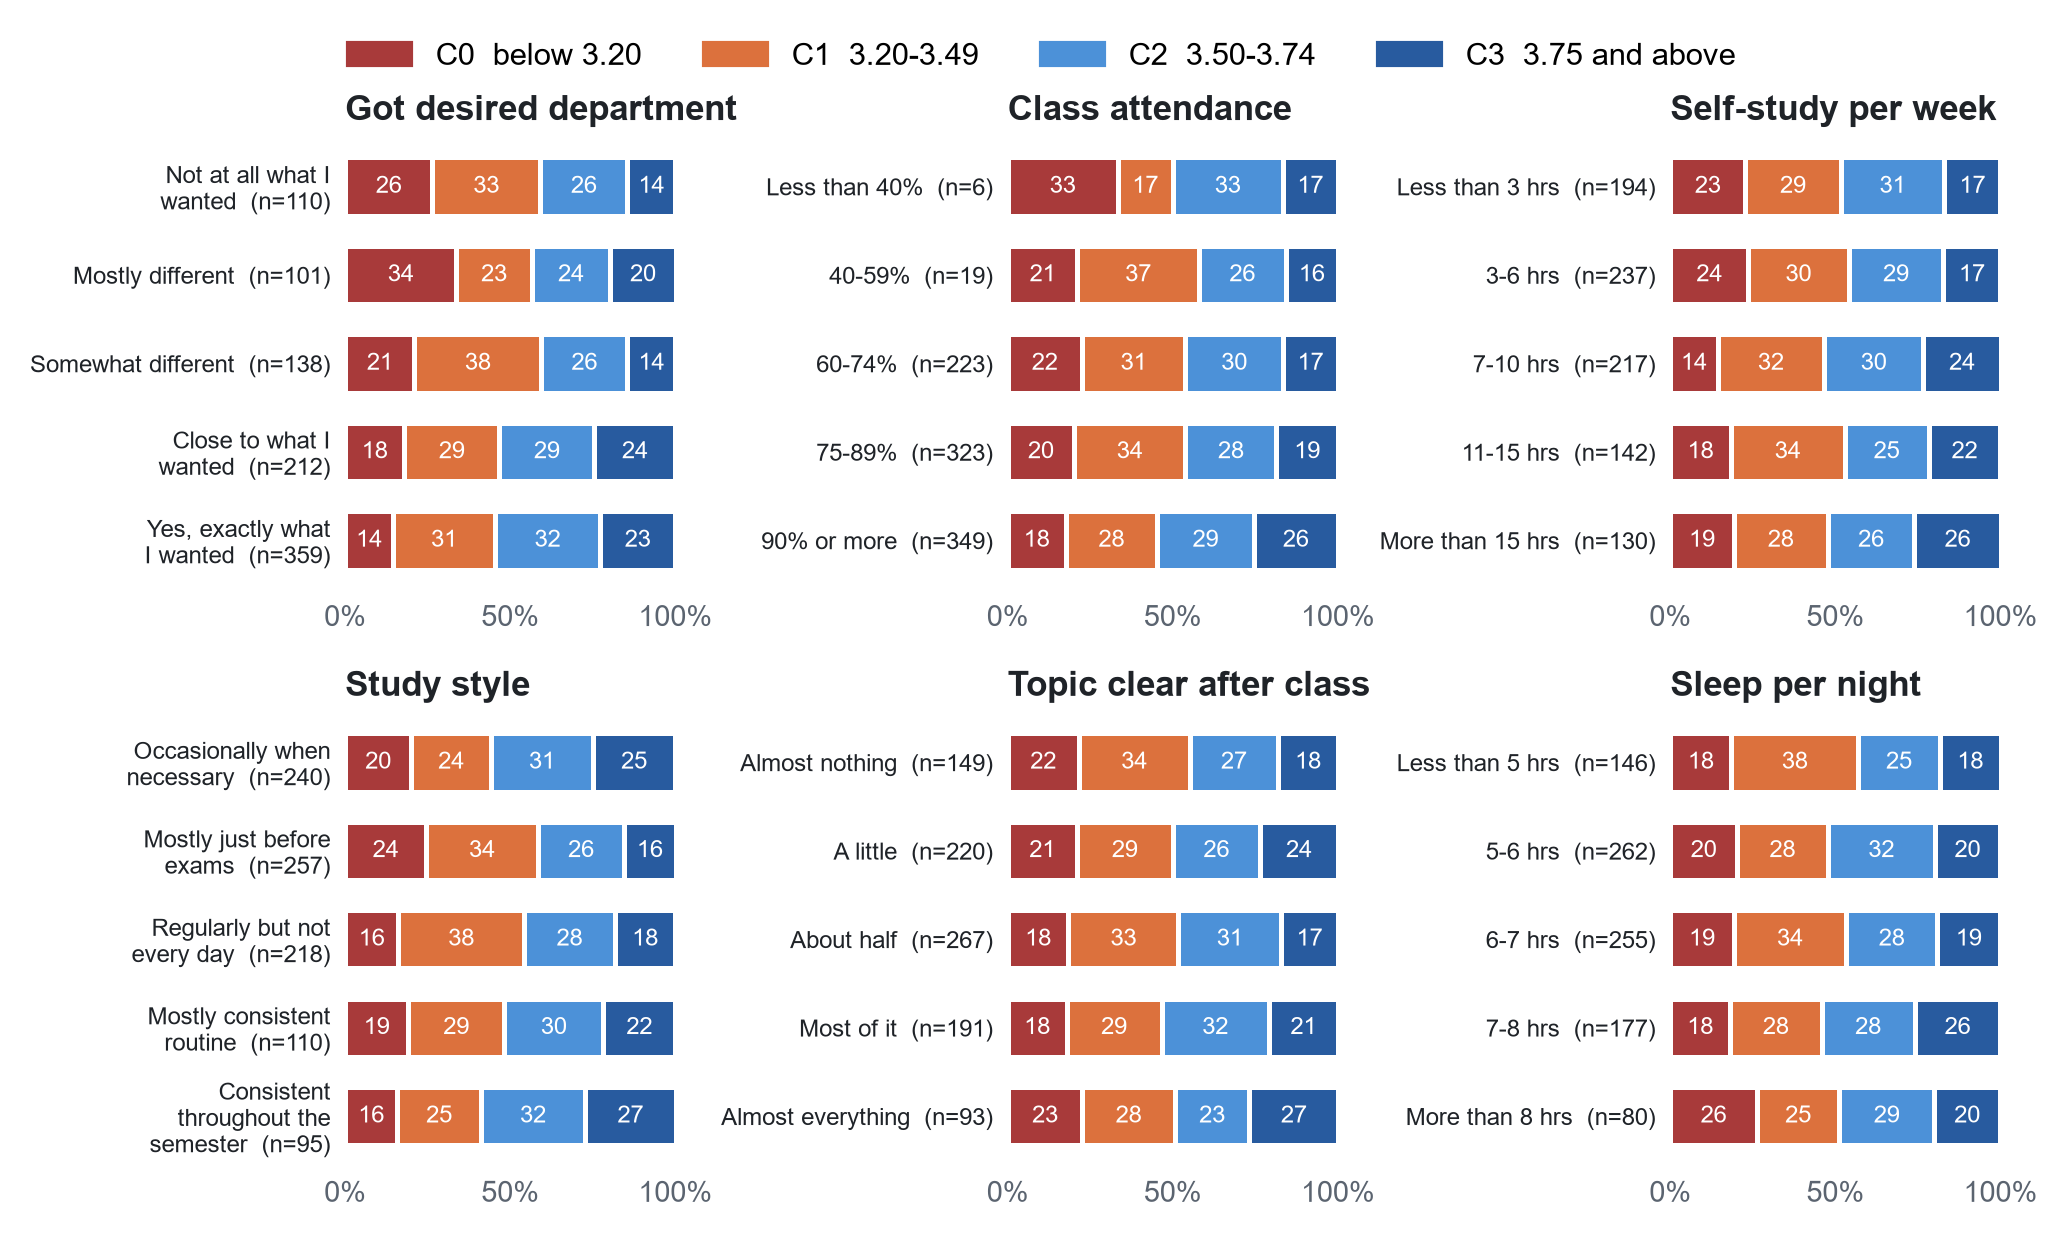
\includegraphics[width=\linewidth]{figures/cgpa_mix_part1.png}
\caption{CGPA-group mix for each answer, questions 1--6. Each bar is 100\% of the students who chose that answer. Numbers inside the bars are percentages; segments under 10\% are not labelled.}
\label{fig:mix1}
\end{figure}

\begin{figure}[!htbp]
\centering
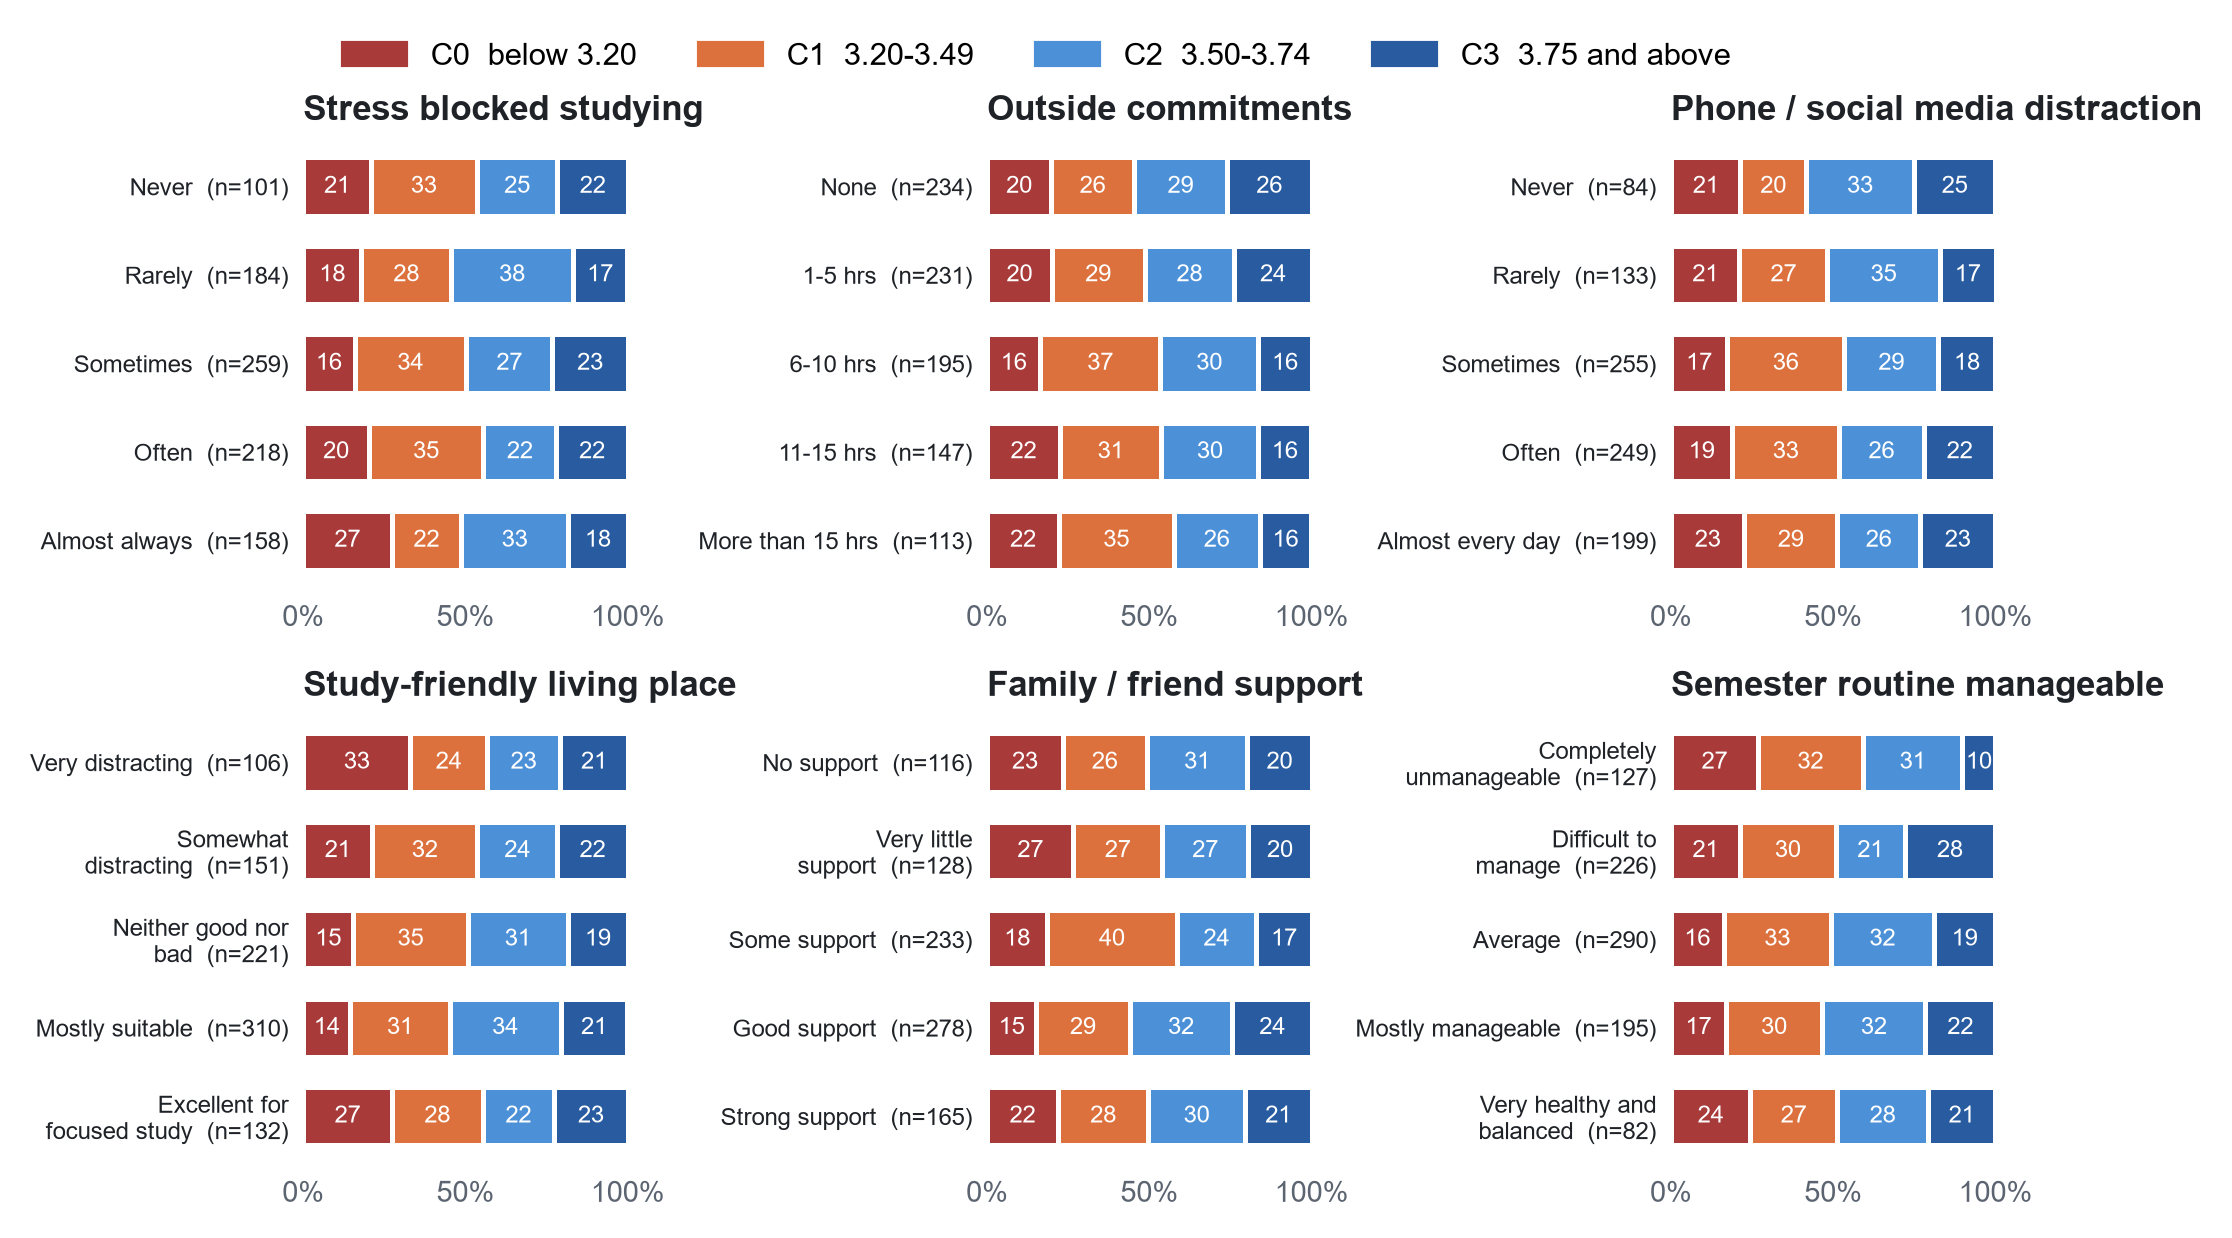
\includegraphics[width=\linewidth]{figures/cgpa_mix_part2.png}
\caption{CGPA-group mix for each answer, questions 7--12. The bars look similar from answer to answer, which is why the questions alone predict the CGPA group only weakly (Section 10.7).}
\label{fig:mix2}
\end{figure}

% =====================================================================================================
\section{8. Data Preprocessing, Curation and Leakage Control}
Every step is scripted. The cleaning, missing-data, outlier, de-identification and leakage rules are applied once to the released files. Only the encoding and the choice of features to leave out are model-specific decisions.

\begin{itemize}
\item \textbf{Cleaning.}
  \begin{itemize}
  \item Each raw column of both forms was mapped by hand to one \texttt{snake\_case} name, with a check that every column is covered.
  \item The Bangla translation in brackets and the emojis were removed from Form B answers, so ``90\% or more'' followed by its Bangla translation becomes ``90\% or more'' (Figure~\ref{fig:rawsheet}); without this step the two forms would share no answer values.
  \item Ten university spellings were reduced to 4 (``BRAC / Brac / BRAc / BRAC University'').
  \item The two department boxes were combined, and 110 department spellings were reduced to 24 departments (``CSE / cse / Computer Science and Egineering''). One unclear entry (``Mecha'') was marked Unknown rather than guessed.
  \item One study-style label written two ways was made the same.
  \item The two grade formats and typed numbers were turned into the four groups C0--C3.
  \item The timestamp and the empty e-mail column were left out of the ML files.
  \item There are no identical duplicate rows: every response has its own timestamp.
  \end{itemize}
\item \textbf{Missing data.}
  \begin{itemize}
  \item Rows with no usable CGPA answer (18, including two ``I don't know'') were removed, because a row without a label cannot be used for training.
  \item Rows whose recent SGPA was blank or unusable (6) were removed from the released ML files. Filling them in would have meant guessing an input from the label.
  \item A blank outside-commitments answer was filled with ``None''. On Form B, where ``None'' was an option, 26.5\% chose it.
  \item Other scattered blanks (under 1.6\% of any question) were filled with the median answer of the same form. We used the median, not the mean, because the answers are ordered categories.
  \item Semester blanks (2) were filled with the median semester of the same university.
  \end{itemize}
\item \textbf{Outliers / noise.} Answers are fixed choices, so there are no impossible values. The noise check compared each student's recent SGPA group with their CGPA group. A gap of two or three groups is possible for a few students, but it is unusual: one semester changes a multi-semester CGPA only a little. Such gaps were concentrated in the KUET semester-7 answers sent on 6--7 August: 182 of 455 answers (40.0\%), against 9.3\% for all other students (Section 9, Table~\ref{tab:gapgroups}). In that batch SGPA and CGPA were unrelated (Spearman $\rho=-0.04$, against $+0.62$ for everyone else). We therefore removed the 182 answers in that batch with a gap of 2--3 groups and kept its other 273 answers. The removed rows are listed in a separate file. Big-gap answers outside that batch (for example 37 at BUET) were kept, because nothing else about them looked unusual.
\item \textbf{Encoding / scaling.} Every five-option answer was coded 0--4 from lowest to highest, keeping the order (Appendix A). The recent SGPA group and the CGPA group are nominal attributes \{C0, C1, C2, C3\} in the ARFF file. No scaling was applied to the released files. WEKA's SMO and Logistic apply their own default normalisation inside each training fold.
\item \textbf{Features left out.} Result satisfaction is left out because it is a subjective reaction to the result, depending on each student's own goals. \texttt{source\_form}, university, department, semester and timestamp are also left out of the model inputs, so the models learn from student answers, not from where or when the form was filled in. Admission satisfaction and career expectation are kept for description only, matching the presentation.
\item \textbf{Augmentation / synthetic data.} None. No row was generated, copied or oversampled.
\item \textbf{De-identification.} The forms collected no names, roll numbers, phone numbers or exact income. The e-mail column was empty and is removed. Timestamps are kept only as a date in the detail file, and university plus department groups are coarse. A few small groups (for example 4 students of one rare BUET department) are reported only as counts.
\item \textbf{Leakage control.}
  \begin{itemize}
  \item The grouping key is the individual response. Each row is a different anonymous student, and nobody was surveyed twice by design.
  \item All cleaning uses fixed rules, not statistics learned from the data, so nothing about a test fold leaks into training.
  \item WEKA's stratified cross-validation places every row in exactly one test fold.
  \item One caveat is stated openly. The removal rule uses the SGPA--CGPA gap, which involves the label, so it is limited to one batch identified by date and semester, and results before the check are always reported next to results after it (Table~\ref{tab:beforeafter}).
  \item The two forms word the CGPA question slightly differently: Form A asks for the CGPA ``before that semester'', and Form B asks for the ``current'' CGPA. So for KUET rows the recent SGPA is partly included in the CGPA. This is listed as a limitation.
  \end{itemize}
\end{itemize}

% =====================================================================================================
\section{9. Technical Validation and Data Quality}
{\small
\begin{tabularx}{\linewidth}{|L{36mm}|Y|}
\hline
\rowcolor{hdr}\hd{Quality dimension} & \hd{Evidence / checks performed} \\ \hline
\hd{Completeness} & 1,126 responses were received and all 1,126 are in the raw files. 1,108 have a usable CGPA and 1,102 also a real recent SGPA. Blank answers per question are counted in Table~\ref{tab:missing}. The released 920 rows have no missing values; the script stops if any remain. \\ \hline
\hd{Consistency} & The column map is checked to cover every raw column. Every answer must match a known option, or the encoding step stops. Answer labels are identical across the two forms after the Bangla text is removed. University and department spellings are standardised. Each response has a unique timestamp, so there are no duplicate submissions. \\ \hline
\hd{Label quality} & Labels are self-reported ranges, not registrar records. We checked them against the linked recent-SGPA question: 78\% of 1,102 students are within one group (Figure~\ref{fig:gap}). Big gaps were concentrated in one batch (Tables~\ref{tab:gapgroups}--\ref{tab:gapsem}). In the final data SGPA and CGPA agree strongly ($\rho=0.65$; Figure~\ref{fig:scatter}). \\ \hline
\hd{Measurement quality} & Single-choice options with fixed ranges prevent impossible values. Questions were bilingual to avoid misreading. Weak points: self-report, and the different time reference of the CGPA question on the two forms. \\ \hline
\hd{Integrity} & Raw exports are kept unchanged. Scripts \texttt{assert} that the 1,108 rows line up one-to-one with the raw timestamps and CGPA answers before any merge. All 67 WEKA logs are stored with their exact commands. \\ \hline
\hd{Representativeness / bias} & KUET is 75\% of rows, and KUET semester 7 dominates it. The sample is convenience-based. Classes are close to balanced (ratio 1.56). CUET has only 25 rows and no C0 student. Gender and income were not collected (Section 12). \\ \hline
\hd{Reproducibility} & \texttt{final\_weka\_results.py} rebuilds the 920-row CSV and ARFF and every WEKA result from the cleaned file. The notebook rebuilds the cleaned file from \texttt{raw-data/}. \texttt{build\_report\_assets.py} rebuilds every table and figure in this report. Seeds are fixed (WEKA \texttt{-s 1}). \\ \hline
\end{tabularx}}

\textbf{The SGPA--CGPA check in detail.} A CGPA averages several semesters, so one semester rarely moves it by more than one group. For example, a student with CGPA 3.80 after five semesters who gets SGPA 2.80 in the sixth semester ends with CGPA 3.63, moving only from C3 to C2. Figure~\ref{fig:gap} shows that 860 of the 1,102 students (78\%) are within one group, and 242 are two or three groups apart. Tables~\ref{tab:gapuni} and \ref{tab:gapsem} show where the big gaps come from. There are none at BRAC or CUET, and almost all KUET big gaps are in semester 7. Within semester 7 they appear on 6--7 August, when 455 answers arrived in two days (Table~\ref{tab:gapgroups}).

\begin{figure}[!htbp]
\centering
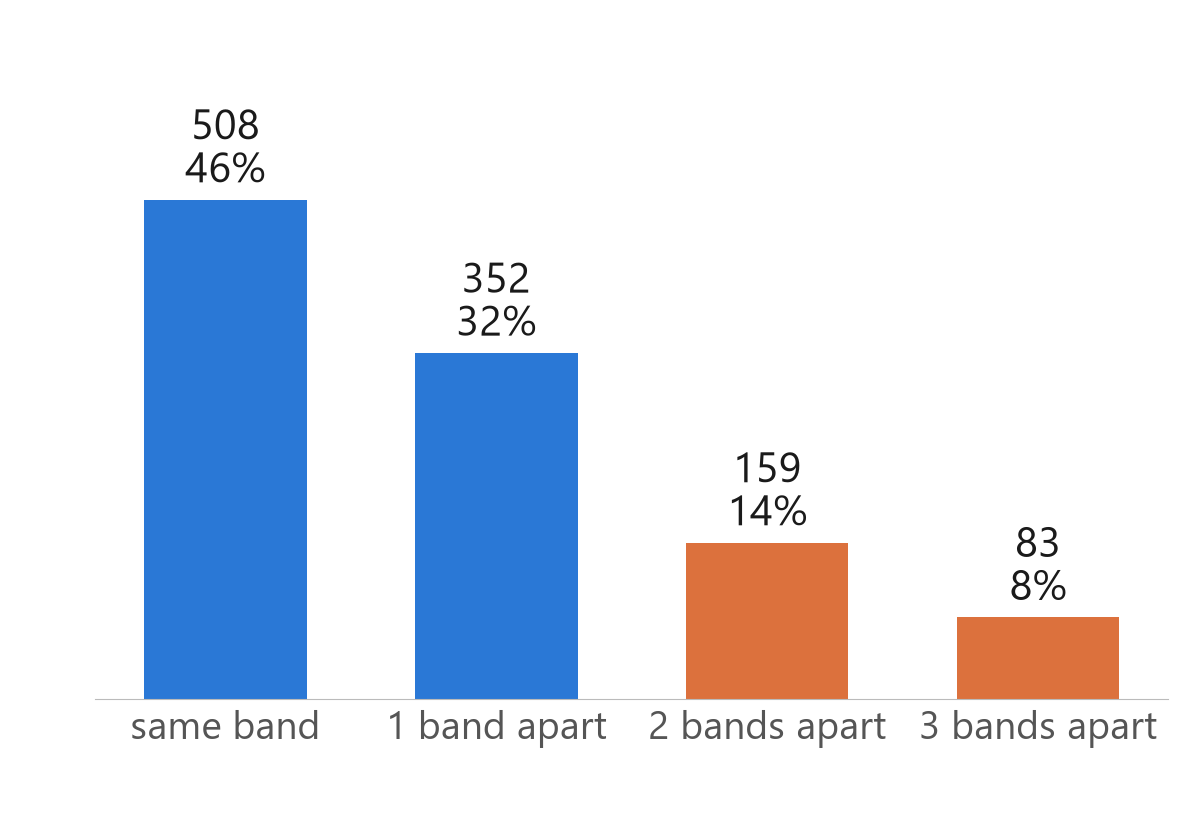
\includegraphics[width=0.6\linewidth]{figures/deck/gap_distribution_1102.png}
\caption{Gap between the recent SGPA group and the CGPA group for the 1,102 rows with both grades. Orange marks a gap of 2--3 groups.}
\label{fig:gap}
\end{figure}

\begin{table}[!htbp]
\centering\small
\caption{Gap between recent SGPA group and CGPA group, by group of rows. $\rho$ is the Spearman correlation between the two grades.}
\label{tab:gapgroups}
\begin{tabularx}{\linewidth}{|Y|R{11mm}|R{11mm}|R{11mm}|R{11mm}|R{11mm}|R{17mm}|R{11mm}|}
\hline
\rowcolor{hdr}\hd{Rows} & \hd{n} & \hd{Gap 0} & \hd{Gap 1} & \hd{Gap 2} & \hd{Gap 3} & \hd{\% gap $\geq$2} & \hd{$\rho$} \\ \hline
\tabinput{tables/gap_groups.tex}
\end{tabularx}
\end{table}

\begin{table}[!htbp]
\centering\small
\begin{minipage}[t]{0.45\linewidth}\centering
\captionof{table}{Big gaps (2--3) by university.}\label{tab:gapuni}
\begin{tabular}{|l|r|r|r|}
\hline
\rowcolor{hdr}\hd{Uni.} & \hd{n} & \hd{Big} & \hd{\%} \\ \hline
\tabinput{tables/gap_university.tex}
\end{tabular}
\end{minipage}\hfill
\begin{minipage}[t]{0.45\linewidth}\centering
\captionof{table}{Big gaps by KUET semester.}\label{tab:gapsem}
\begin{tabular}{|c|r|r|r|}
\hline
\rowcolor{hdr}\hd{Sem} & \hd{n} & \hd{Big} & \hd{\%} \\ \hline
\tabinput{tables/gap_kuet_semester.tex}
\end{tabular}
\end{minipage}
\end{table}

\begin{figure}[!htbp]
\centering
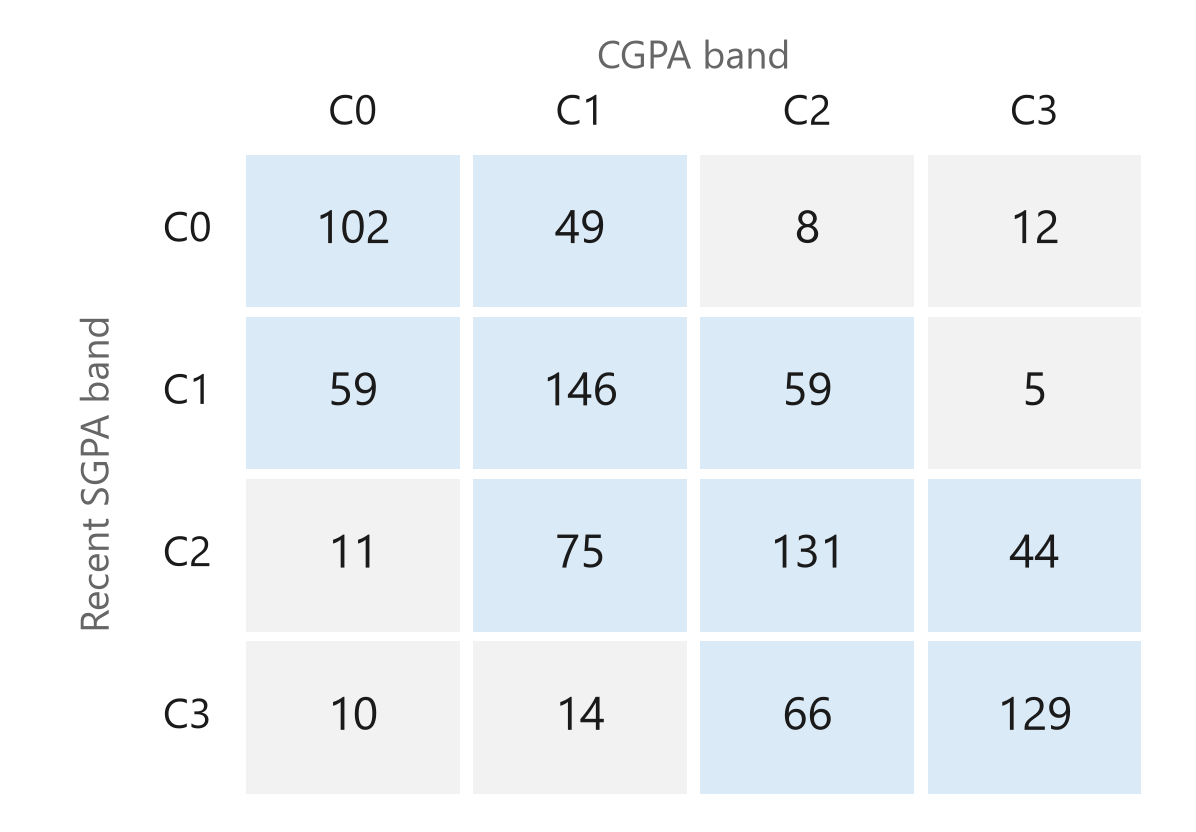
\includegraphics[width=0.6\linewidth]{figures/deck/sgpa_x_cgpa_final.png}
\caption{Recent SGPA group (rows) against CGPA group (columns) for the 920 students in the final dataset. Blue cells are the same group or one group apart (860 students, 93.5\%).}
\label{fig:scatter}
\end{figure}

The 182 removed answers are 121 with a gap of two groups and 61 with a gap of three. In 92 the SGPA is lower than the CGPA and in 90 it is higher, so the removal does not favour better or worse students. By date, 131 were sent on 6 August and 51 on 7 August. Because the removed rows are split almost evenly between ``SGPA too low'' and ``SGPA too high'', the removal does not shift the CGPA distribution towards one end (C0 54, C1 36, C2 36, C3 56 removed). Table~\ref{tab:sgcg} shows the agreement of the two grades in the released data.

\begin{table}[!htbp]
\centering\small
\caption{Recent SGPA group against CGPA group in the released 920 rows. Blue cells: same group (508 students, 55.2\%); a further 352 (38.3\%) are one group apart.}
\label{tab:sgcg}
\begin{tabular}{|l|c|c|c|c|r|}
\hline
\rowcolor{hdr} & \hd{CGPA C0} & \hd{CGPA C1} & \hd{CGPA C2} & \hd{CGPA C3} & \hd{Total} \\ \hline
\tabinput{tables/sgpa_cgpa_final.tex}
\end{tabular}
\end{table}

\subsection{9.1 Comparison with Existing Datasets and Significance}
Table~\ref{tab:compare} compares our dataset with public student-performance datasets that are often used in machine learning courses and papers, and with the Bangladeshi studies cited in our presentation.

\begin{table}[!htbp]
\centering\footnotesize
\caption{Comparison with related datasets. Figures are as reported by the dataset authors.}
\label{tab:compare}
\begin{tabularx}{\linewidth}{|L{30mm}|L{30mm}|R{12mm}|L{22mm}|Y|L{22mm}|}
\hline
\rowcolor{hdr}\hd{Dataset} & \hd{Population / place} & \hd{Records} & \hd{Features} & \hd{Target} & \hd{Collection / access} \\ \hline
UCI Student Performance [4] & Two secondary schools, Portugal & 649 + 395 & 30 attributes + 3 grades & Final grade G3 (0--20) & School reports and questionnaire; UCI, open \\ \hline
Predict Students' Dropout and Academic Success [5] & One higher-education institution, Portugal & 4,424 & 36 & Dropout / enrolled / graduate & Administrative records; UCI, open \\ \hline
Higher Education Students Performance Evaluation [6] & Engineering and education faculties, Cyprus & 145 & 31 & Course grade (8 classes) & Questionnaire; UCI, open \\ \hline
xAPI-Edu-Data [7] & Kalboard 360 learning platform users & 480 & 16 & Low / middle / high & LMS logs and parent survey; open \\ \hline
Maruf et al.\ [2]; Albonny and Duru [3] & Bangladeshi SSC/HSC and secondary-school students & -- & -- & Exam results; average course grade & Studies; data not released with a data descriptor \\ \hline
\textbf{This dataset} & \textbf{Engineering undergraduates at 4 universities, Bangladesh} & \textbf{1,126 raw; 920 final} & \textbf{12 behaviour answers + recent SGPA (15 answers + context in detail file)} & \textbf{CGPA group C0--C3} & \textbf{Bilingual Google Forms; raw + processed + removal list; GitHub} \\ \hline
\end{tabularx}
\end{table}

\textbf{Novelty and significant properties.}
\begin{itemize}
\item It is, to our knowledge, the first openly documented dataset linking study habits and well-being to CGPA for \emph{engineering undergraduates in Bangladesh}, across four universities.
\item It is a large primary sample compared with similar questionnaire datasets: 920 checked rows against 145 in [6].
\item Raw bilingual exports, cleaned files, the list of removed rows and the scripts are released together, so every cleaning decision can be checked or reversed.
\item It includes a documented label check (SGPA against CGPA) that finds a batch of unreliable answers. This is useful teaching material on survey data quality [16], which most public datasets do not provide.
\item All answers use fixed five-level codes with published meanings, and the files load directly in WEKA (ARFF) or Python (CSV).
\end{itemize}

% =====================================================================================================
\section{10. Machine Learning (ML) Use Demonstration}
\subsection{10.1 ML task definition}
\textbf{Task:} four-class classification (the classes are ordered). \textbf{Input $X$:} the 12 coded answers (numeric 0--4) and \texttt{recent\_sgpa\_band} (nominal C0--C3). \textbf{Target $y$:} \texttt{cgpa\_band} (C0--C3). \textbf{Unit of prediction:} one student. \textbf{Practical output:} the student's likely CGPA group, with readable J48 rules. Two extra experiments on the same 920 rows show how much the questions carry on their own: the questions only, predicting the CGPA group, and the questions only, predicting the recent SGPA group.

\subsection{10.2 Data partitioning strategy}
The main evaluation is WEKA's \textbf{stratified 5-fold cross-validation} with random seed 1 (\texttt{-x 5 -s 1}). Each of the 920 students is tested exactly once, by a model that did not see them in training, and each fold keeps the class proportions. As a backup, WEKA's \textbf{80/20 percentage split} with seed 1 (\texttt{-split-percentage 80 -s 1}) trains on 736 students and tests on 184. Its test set has 35, 66, 46 and 37 students in C0--C3. No separate validation set was used, because no hyperparameter was tuned on the test data: J48's minimum leaf size of 40 was fixed so the tree stays small and readable. Leakage safety: every row is a different student, and no statistic is fitted before splitting (Section 8).

\subsection{10.3 Preprocessing and feature/representation steps}
The ML files use exactly the fixed coding in Appendix A. No step is fitted on the data before splitting. Inside WEKA, SMO normalises numeric inputs to 0--1 and converts the nominal SGPA group to binary indicators. Logistic applies the same indicator coding. Both steps are recomputed on each training fold by WEKA. J48, Random Forest, OneR and Naive Bayes use the attributes as they are.

\subsection{10.4 ML model(s) and hyperparameters}
All models use WEKA 3.8.7 [8]. ZeroR (always predicts the largest class) is the baseline.
\begin{itemize}
\item \textbf{J48} (C4.5 decision tree [9]): \texttt{-C 0.25 -M 40} (confidence 0.25, at least 40 students per leaf).
\item \textbf{Random Forest} [10]: \texttt{-P 100 -I 100 -num-slots 1 -K 0 -M 1.0 -V 0.001 -S 1} (100 trees).
\item \textbf{SMO} (support vector machine [11]): WEKA defaults (C = 1.0, linear polynomial kernel, inputs normalised).
\item \textbf{Logistic regression} [12]: \texttt{-R 1.0E-8 -M -1}.
\item \textbf{Naive Bayes} [13] and \textbf{OneR} [14] (\texttt{-B 6}): WEKA defaults.
\end{itemize}

\subsection{10.5 Evaluation metrics}
The four classes are close to balanced, so \textbf{accuracy} is a fair main metric, always compared with the ZeroR baseline (30.87\%). We also report:
\begin{itemize}
\item \textbf{Cohen's kappa} [17]: agreement beyond chance.
\item \textbf{Macro-F1}: every class counts equally, so the smallest group C0 is not ignored.
\item \textbf{Weighted F1}.
\item \textbf{Within-one-group rate}: the share of predictions no more than one CGPA group away from the truth, which matters because the classes are ordered.
\item The \textbf{confusion matrix}.
\end{itemize}

\subsection{10.6 Reproducibility}
\begin{itemize}
\item \textbf{Environment.} Windows 11; Python 3.14.5 in the project \texttt{venv}; WEKA 3.8.7 with its bundled Java runtime (flag \texttt{--add-opens java.base/java.lang=ALL-UNNAMED}).
\item \textbf{Scripts.} \texttt{notebooks/final\_weka\_results.py} builds \texttt{final\_920.csv/.arff}, runs all 7 models $\times$ 3 experiments $\times$ \{5-fold CV, 80/20 split\}, and writes the logs to \texttt{docs/weka\_runs/final/} and the numbers to \texttt{docs/final\_results.json}.
\item \textbf{Manual check.} \texttt{docs/FINAL\_WEKA\_STEPS.md} explains how to repeat every result in the WEKA Explorer (Classify tab, Cross-validation, Folds = 5, seed = 1).
\item \textbf{Seeds.} Random seed 1 for cross-validation, the split and Random Forest.
\item \textbf{Hardware.} An ordinary laptop; every run takes seconds.
\end{itemize}

\subsection{10.7 Results (compact)}
\begin{table}[!htbp]
\centering\small
\caption{WEKA results on the 920 rows, stratified 5-fold cross-validation, seed 1. Main task: 12 answers + recent SGPA group $\rightarrow$ CGPA group. The last two columns give accuracy when only the 12 answers are used.}
\label{tab:results}
\begin{tabularx}{\linewidth}{|Y|R{14mm}|R{11mm}|R{13mm}|R{15mm}|R{15mm}|R{17mm}|R{17mm}|}
\hline
\rowcolor{hdr}\hd{Model} & \hd{Accuracy \%} & \hd{Kappa} & \hd{Macro-F1} & \hd{Weighted F1} & \hd{Within 1 group \%} & \hd{Answers only $\rightarrow$ CGPA \%} & \hd{Answers only $\rightarrow$ SGPA \%} \\ \hline
\tabinput{tables/weka_cv5.tex}
\end{tabularx}
\end{table}

\begin{table}[!htbp]
\centering\small
\begin{minipage}[t]{0.47\linewidth}\centering
\captionof{table}{Main task, 5-fold CV, before and after the data check (same models and settings).}\label{tab:beforeafter}
\begin{tabular}{|l|r|r|}
\hline
\rowcolor{hdr}\hd{Model} & \hd{1,102 rows} & \hd{920 rows} \\ \hline
ZeroR & 29.04 & 30.87 \\ \hline
J48 & 43.56 & 54.35 \\ \hline
Random Forest & 45.01 & 54.24 \\ \hline
SMO & 46.10 & \textbf{55.22} \\ \hline
Logistic & 46.37 & 54.67 \\ \hline
Naive Bayes & 44.83 & 54.46 \\ \hline
\end{tabular}
\end{minipage}\hfill
\begin{minipage}[t]{0.50\linewidth}\centering
\captionof{table}{Confusion matrix, SMO, main task, 5-fold CV (rows actual, columns predicted; blue = correct).}\label{tab:cm}
\begin{tabular}{|l|c|c|c|c|r|}
\hline
\rowcolor{hdr} & \hd{C0} & \hd{C1} & \hd{C2} & \hd{C3} & \hd{Total} \\ \hline
\tabinput{tables/cm_smo_cv5.tex}
\end{tabular}
\end{minipage}
\end{table}

\begin{table}[!htbp]
\centering\small
\caption{Backup check: WEKA 80/20 percentage split, seed 1 (736 training, 184 test students). With only 184 test students these numbers move more than the cross-validation results.}
\label{tab:split}
\begin{tabular}{|l|r|r|r|r|}
\hline
\rowcolor{hdr}\hd{Model} & \hd{Main accuracy \%} & \hd{Kappa} & \hd{Answers only $\rightarrow$ CGPA \%} & \hd{Answers only $\rightarrow$ SGPA \%} \\ \hline
\tabinput{tables/weka_split80.tex}
\end{tabular}
\end{table}

\textbf{What this shows about dataset usability.}
\begin{itemize}
\item The released data supports a working WEKA pipeline. Every model beats the 30.87\% baseline by more than 23 points on the main task, with kappa about 0.38--0.40, and 93\% of SMO's predictions are within one CGPA group.
\item The best models (SMO 55.22\%, Logistic 54.67\%, J48 54.35\%) are close together, so the result does not depend on one algorithm.
\item The J48 tree with at least 40 students per leaf uses only the recent SGPA group: one rule per group (Figure~\ref{fig:tree}). The same tree with WEKA's default leaf size of 2 grows to 175 leaves and scores only 46.52\%.
\item With the answers alone, every model stays near the baseline (27.8--33.8\%). The habits in this questionnaire relate to CGPA only weakly (Section 7.3.3), which is itself a useful finding for anyone reusing the data.
\item The data check raised every model by about 8--11 points (Table~\ref{tab:beforeafter}), which shows how much careless answers can hide.
\end{itemize}
We do not claim these models are good enough to decide anything about an individual student.

\begin{figure}[!htbp]
\centering
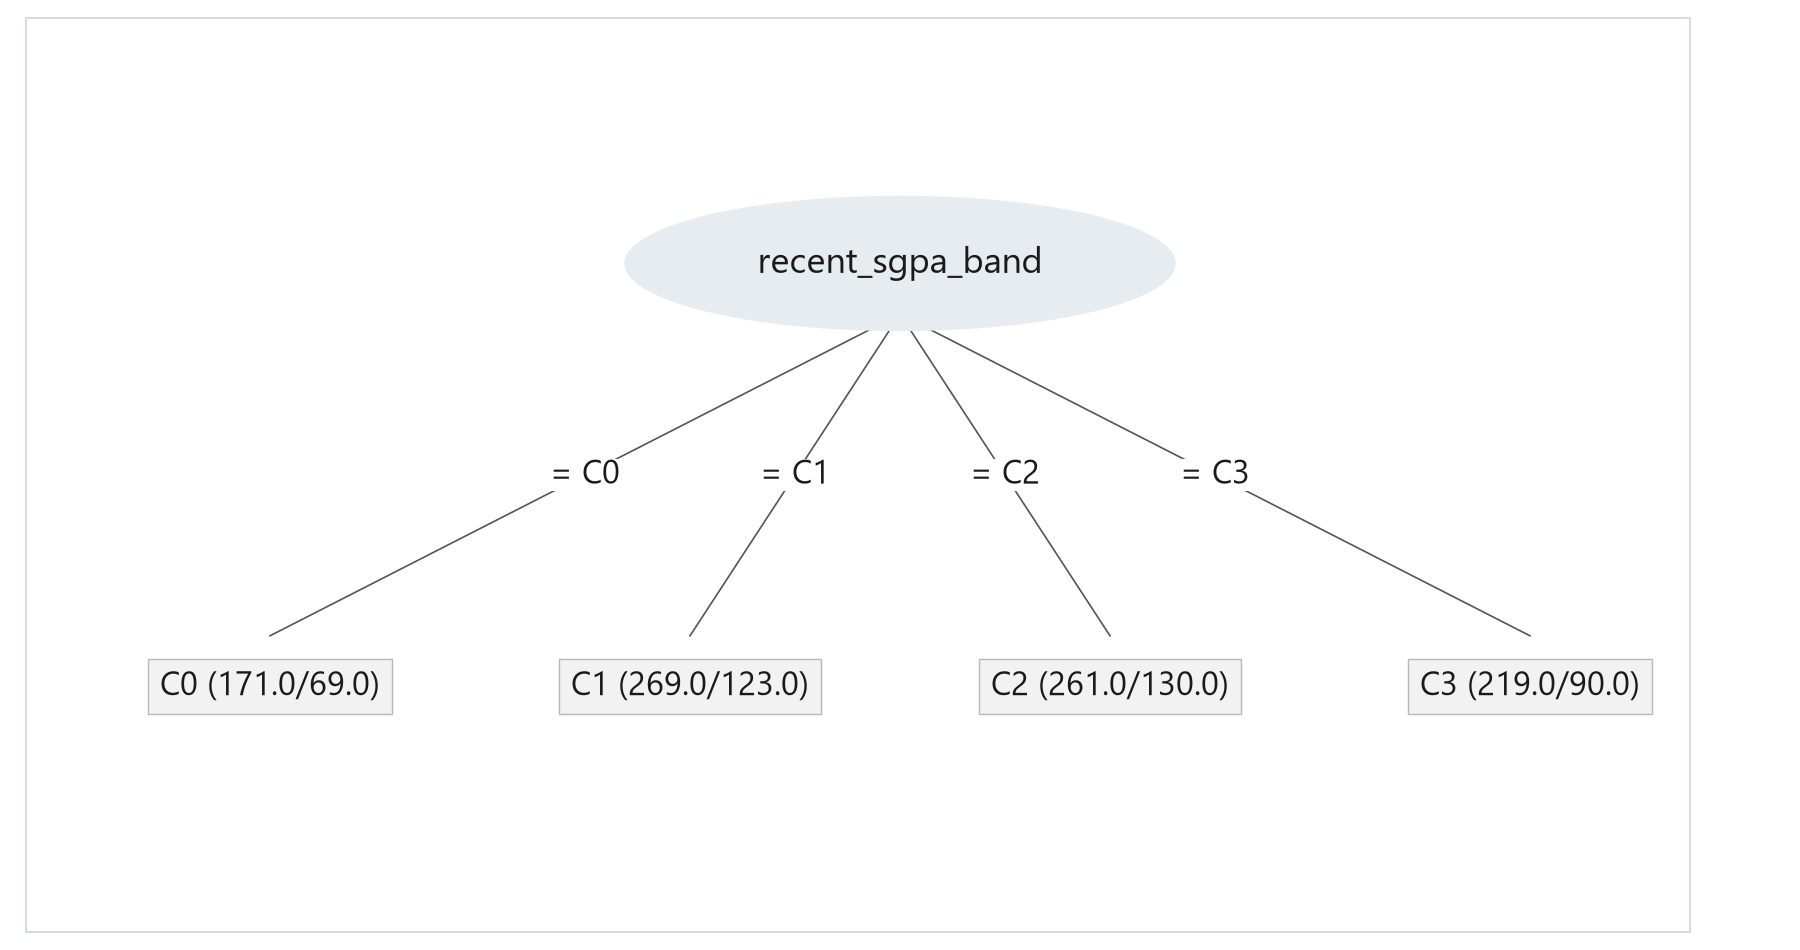
\includegraphics[width=0.62\linewidth]{figures/deck/tree_main_cgpa.png}
\caption{WEKA J48 tree for the main task, built on all 920 students (\texttt{-C 0.25 -M 40}). Leaf labels show (students in leaf / students placed in the wrong group).}
\label{fig:tree}
\end{figure}

% =====================================================================================================
\section{11. Usage Notes and Reuse Potential}
\begin{itemize}
\item \textbf{Download and load.} Clone or download the GitHub repository. In WEKA: Explorer $\rightarrow$ Preprocess $\rightarrow$ Open file $\rightarrow$ \texttt{cleaned-dataset/ours/final/final\_920.arff} (it should show 920 instances and 14 attributes); the class is \texttt{cgpa\_band}. In Python: \texttt{pandas.read\_csv("final\_920.csv")}. When reading the detail file, keep ``None'' as text (\texttt{keep\_default\_na=False}).
\item \textbf{Software.} WEKA 3.8.x, or any CSV reader. Rebuilding the files needs Python 3.14 with pandas, NumPy and SciPy (versions in Section 3).
\item \textbf{Coding conventions.} Answers are coded 0 (lowest option) to 4 (highest option); \texttt{answer\_codes.csv} gives each meaning. For study style, 0 is ``Occasionally when necessary'' and 1 is ``Mostly just before exams''. Groups C0--C3 use the cut-points 3.20, 3.50 and 3.75. Use the ARFF rather than the CSV in WEKA, so the class order C0--C3 is fixed.
\item \textbf{Precautions.}
  \begin{itemize}
  \item KUET semester 7 dominates the sample.
  \item The CGPA question has a different time reference on the two forms.
  \item Grades are self-reported ranges.
  \item Use stratified cross-validation, and report ZeroR next to any accuracy.
  \item Do not use \texttt{source\_form}, university or date as model inputs if the aim is to learn about student behaviour.
  \end{itemize}
\item \textbf{Potential reuse.} Ordinal classification methods; cost-sensitive learning where a two-group error counts more; clustering of student habit profiles; comparing universities with the detail file; careless-response detection with \texttt{dropped\_182\_rows.csv}; extending the survey to more universities or semesters with the same codes.
\item \textbf{Misleading uses.}
  \begin{itemize}
  \item Do not read the associations as causes (for example ``attending more will raise your CGPA'').
  \item Do not rank individual students or make admission, scholarship or disciplinary decisions from these models.
  \item Do not generalise to non-engineering or non-Bangladeshi students without new data.
  \end{itemize}
\end{itemize}

% =====================================================================================================
\section{12. Limitations and Known Biases}
\begin{itemize}
\item \textbf{Self-report.} All answers, including grades, are self-reported and were not checked against registrar records.
\item \textbf{Convenience sample.} The sample is KUET-heavy (75\%, mostly semester 7), so results may not describe other years or universities. CUET (25 rows) and several departments are very small.
\item \textbf{Grade format.} Grades are ranges, so small differences inside a group are lost. The CGPA question refers to ``before that semester'' on Form A and ``current'' on Form B.
\item \textbf{Data check.} The check removed only the clearest unreliable answers (182). Some kept answers may still be careless, and some removed answers may have been honest.
\item \textbf{Satisfaction answers.} KUET students gave many ``Very dissatisfied'' answers to the admission and result satisfaction questions (360 and 387 of 896 raw answers). These may reflect real feelings or the order in which the options were shown, so they are not used as model inputs.
\item \textbf{Missing context.} Gender, family income and school background were not collected, so bias along these lines cannot be checked.
\item \textbf{One point in time.} The survey was a single round, so changes over time cannot be studied.
\end{itemize}

% =====================================================================================================
\section{13. Ethics, Privacy and Responsible Data Use}
{\small
\begin{tabularx}{\linewidth}{|L{55mm}|Y|}
\hline
\hd{Human participants / consent} & Adult university students took part voluntarily and anonymously in a course project. The form's opening text explained the purpose and stated that the survey was anonymous. Submitting the form was taken as consent. No institutional ethics-board approval was requested for this course project. \\ \hline
\hd{Privacy / de-identification} & No names, roll numbers, phone numbers or exact income were collected. The e-mail column (empty) was removed. Released files keep only university, department, semester and the submission date, and results for very small groups are shown only as counts. \\ \hline
\hd{Web / social-media data} & Not applicable. Form links were shared in student groups, but no content was collected from social-media platforms. \\ \hline
\hd{Copyright / third-party data} & All questions and answers were created and collected by the group. Google Forms was used as a tool only. Figures of related datasets are cited from their authors [4]--[7]. \\ \hline
\hd{AI-generated / synthetic content} & No synthetic or AI-generated data are in the dataset: 0\% of rows. An AI coding assistant (Claude, Anthropic) helped write cleaning and analysis scripts and draft documentation text. All numbers come from the scripts and WEKA logs in the repository and were reviewed by the group. \\ \hline
\end{tabularx}}

% =====================================================================================================
\section{14. Data and Code Availability}
{\small
\begin{tabularx}{\linewidth}{|L{55mm}|Y|}
\hline
\rowcolor{hdr}\hd{Item} & \hd{Details} \\ \hline
\hd{Repository name} & GitHub (\texttt{SheikhGalib/CGPA-does-matter-dataset-ml-lab}) \\ \hline
\hd{Dataset DOI / persistent identifier} & Not yet assigned (a Zenodo archive of release v1.0 is planned) \\ \hline
\hd{Direct dataset URL} & \url{https://github.com/SheikhGalib/CGPA-does-matter-dataset-ml-lab/tree/main/cleaned-dataset/ours/final} \\ \hline
\hd{Access instructions} & Access through the repository link; contact the corresponding student if the repository is private at the time of reading \\ \hline
\hd{Dataset license} & CC BY 4.0 (proposed) \\ \hline
\hd{Code / notebook URL} & \url{https://github.com/SheikhGalib/CGPA-does-matter-dataset-ml-lab} (\texttt{notebooks/}, \texttt{report/build\_report\_assets.py}) \\ \hline
\hd{Code version / commit / release} & v1.0; commit \texttt{32ce1ce} (15 September 2026) \\ \hline
\hd{README \& environment} & \texttt{AGENTS.md} (project README), \texttt{docs/FINAL\_WEKA\_STEPS.md} (WEKA guide); Python 3.14.5, pandas 3.0.5, NumPy 2.5.2, SciPy 1.18.1, matplotlib 3.11.1; WEKA 3.8.7 \\ \hline
\end{tabularx}}

% =====================================================================================================
\section{15. Student Contributions (CRediT-style)}
{\small
\begin{tabularx}{\linewidth}{|L{15mm}|L{32mm}|C{16mm}|Y|L{38mm}|}
\hline
\rowcolor{hdr}\hd{Roll} & \hd{Student} & \hd{Overall Contribution (\%)} & \hd{Main contributions} & \hd{Evidence / files owned} \\ \hline
2107020 & Sheikh Md.\ Galib Mahim & 16.67 & Data curation, software, formal analysis, visualization, writing -- original draft & Merge and cleaning notebook, final data check, WEKA pipeline, report \\ \hline
2107030 & Md.\ Eftakar Jaman Arfan & 16.67 & Investigation, validation, formal analysis & WEKA experiments and result tables \\ \hline
2107007 & Asif Jawad & 16.67 & Conceptualization, methodology, investigation (data collection) & Form design and data collection \\ \hline
2107008 & Rakibul Islam & 16.67 & Writing -- review and editing; literature review & Report writing, related work \\ \hline
2107012 & Md Enam E Elahi & 16.67 & Writing -- review and editing; literature review & Report writing, related work \\ \hline
2107014 & Al Mubtasim Preom & 16.67 & Data curation & Cleaning of the KUET form scheme \\ \hline
\end{tabularx}}

% =====================================================================================================
\section{16. Acknowledgements, Funding and Competing Interests}
\subsection{16.1 Acknowledgements / Funding}
We thank every student at KUET, BUET, BRAC University and CUET who answered the forms, and the classmates who shared the links. We thank the CSE 4112 course teachers for their guidance. This work received no external funding.

\subsection{16.2 Declaration of Competing Interests}
The authors declare no competing interests relevant to this dataset report.

% =====================================================================================================
\section{17. References}
{\small
\begin{enumerate}[label={[\arabic*]},leftmargin=22pt,itemsep=2pt]
\item Ahmed, study of student performance classification using K-means clustering with SVM, decision tree, naive Bayes and KNN, 2024, DOI: \url{https://doi.org/10.1155/2024/4067721}.
\item Maruf et al., machine-learning prediction of SSC and HSC results in Bangladesh with a stacking ensemble, Proc.\ ICCIT 2024, DOI: \url{https://doi.org/10.1109/ICCIT64611.2024.11021990}.
\item Albonny and Duru, prediction of the average course grade of Bangladeshi secondary-school students with regression, tree, random forest and deep neural network models, International Journal of Engineering, Science and Technology (IJONFEST), 2026, URL: \url{https://dergipark.org.tr/tr/pub/ijonfest/article/1879280}.
\item P. Cortez and A. Silva, ``Using data mining to predict secondary school student performance,'' in Proc.\ 5th Future Business Technology Conference (FUBUTEC 2008), pp.\ 5--12, 2008. Dataset: UCI Machine Learning Repository, DOI: \url{https://doi.org/10.24432/C5TG7T}.
\item V. Realinho, J. Machado, L. Baptista and M. V. Martins, ``Predicting student dropout and academic success,'' Data, vol.\ 7, no.\ 11, art.\ 146, 2022, DOI: \url{https://doi.org/10.3390/data7110146}.
\item N. Yılmaz and B. Sekeroglu, ``Student performance classification using artificial intelligence techniques,'' in Proc.\ ICSCCW 2019, Springer, 2020, DOI: \url{https://doi.org/10.1007/978-3-030-35249-3_76}.
\item E. A. Amrieh, T. Hamtini and I. Aljarah, ``Mining educational data to predict student's academic performance using ensemble methods,'' International Journal of Database Theory and Application, vol.\ 9, no.\ 8, pp.\ 119--136, 2016, DOI: \url{https://doi.org/10.14257/ijdta.2016.9.8.13}.
\item M. Hall, E. Frank, G. Holmes, B. Pfahringer, P. Reutemann and I. H. Witten, ``The WEKA data mining software: an update,'' SIGKDD Explorations, vol.\ 11, no.\ 1, pp.\ 10--18, 2009, DOI: \url{https://doi.org/10.1145/1656274.1656278}.
\item J. R. Quinlan, C4.5: Programs for Machine Learning. San Mateo, CA: Morgan Kaufmann, 1993.
\item L. Breiman, ``Random forests,'' Machine Learning, vol.\ 45, pp.\ 5--32, 2001, DOI: \url{https://doi.org/10.1023/A:1010933404324}.
\item J. C. Platt, ``Fast training of support vector machines using sequential minimal optimization,'' in Advances in Kernel Methods: Support Vector Learning, MIT Press, 1999, pp.\ 185--208.
\item S. le Cessie and J. C. van Houwelingen, ``Ridge estimators in logistic regression,'' Applied Statistics, vol.\ 41, no.\ 1, pp.\ 191--201, 1992, DOI: \url{https://doi.org/10.2307/2347628}.
\item G. H. John and P. Langley, ``Estimating continuous distributions in Bayesian classifiers,'' in Proc.\ 11th Conference on Uncertainty in Artificial Intelligence, pp.\ 338--345, 1995.
\item R. C. Holte, ``Very simple classification rules perform well on most commonly used datasets,'' Machine Learning, vol.\ 11, pp.\ 63--91, 1993, DOI: \url{https://doi.org/10.1023/A:1022631118932}.
\item Y. Benjamini and Y. Hochberg, ``Controlling the false discovery rate: a practical and powerful approach to multiple testing,'' Journal of the Royal Statistical Society B, vol.\ 57, no.\ 1, pp.\ 289--300, 1995, DOI: \url{https://doi.org/10.1111/j.2517-6161.1995.tb02031.x}.
\item A. W. Meade and S. B. Craig, ``Identifying careless responses in survey data,'' Psychological Methods, vol.\ 17, no.\ 3, pp.\ 437--455, 2012, DOI: \url{https://doi.org/10.1037/a0028085}.
\item J. Cohen, ``A coefficient of agreement for nominal scales,'' Educational and Psychological Measurement, vol.\ 20, no.\ 1, pp.\ 37--46, 1960, DOI: \url{https://doi.org/10.1177/001316446002000104}.
\item M. D. Wilkinson et al., ``The FAIR Guiding Principles for scientific data management and stewardship,'' Scientific Data, vol.\ 3, art.\ 160018, 2016, DOI: \url{https://doi.org/10.1038/sdata.2016.18}.
\end{enumerate}}

% =====================================================================================================
\newpage
\section{Appendix A. Complete Data Dictionary}
Released ML files \texttt{final\_920.csv} / \texttt{final\_920.arff} contain the first 14 fields. \texttt{final\_920\_with\_details.csv} adds the context fields and the answer text (one \texttt{\_code} column per question). Answer codes are listed from 0 to 4.

{\footnotesize
\setlength{\tabcolsep}{3pt}
\begin{longtable}{|L{39mm}|L{33mm}|L{12mm}|L{58mm}|L{17mm}|}
\hline
\rowcolor{hdr}\hd{Field} & \hd{Question / meaning} & \hd{Type} & \hd{Codes (0 $\rightarrow$ 4) or values} & \hd{Missing rule} \\ \hline
\endfirsthead
\hline
\rowcolor{hdr}\hd{Field} & \hd{Question / meaning} & \hd{Type} & \hd{Codes (0 $\rightarrow$ 4) or values} & \hd{Missing rule} \\ \hline
\endhead
\multicolumn{5}{|l|}{\cellcolor{qhead}\textbf{Model inputs (in \texttt{final\_920.csv} and \texttt{.arff})}} \\ \hline
\texttt{desired\_department\_match} & Got into desired subject or department & ordinal 0--4 & Not at all what I wanted; Mostly different; Somewhat different; Close to what I wanted; Yes, exactly what I wanted & form median \\ \hline
\texttt{attendance} & How often present in class & ordinal 0--4 & Less than 40\%; 40--59\%; 60--74\%; 75--89\%; 90\% or more & form median \\ \hline
\texttt{weekly\_study\_time} & Self-study outside class per week & ordinal 0--4 & Less than 3 hrs; 3--6 hrs; 7--10 hrs; 11--15 hrs; More than 15 hrs & form median \\ \hline
\texttt{study\_style} & Study style that fits best & ordinal 0--4 & Occasionally when necessary; Mostly just before exams; Regularly but not every day; Mostly consistent routine; Consistent throughout the semester & form median \\ \hline
\texttt{topic\_clarity} & How much of the topic was clear after class & ordinal 0--4 & Almost nothing; A little; About half; Most of it; Almost everything & form median \\ \hline
\texttt{sleep\_duration} & Sleep on a normal night & ordinal 0--4 & Less than 5 hrs; 5--6 hrs; 6--7 hrs; 7--8 hrs; More than 8 hrs & form median \\ \hline
\texttt{stress\_frequency} & How often stress made studying difficult & ordinal 0--4 & Never; Rarely; Sometimes; Often; Almost always & form median \\ \hline
\texttt{weekly\_\allowbreak responsibilities} & Weekly hours on tuition, job, clubs, other duties & ordinal 0--4 & None; 1--5 hrs; 6--10 hrs; 11--15 hrs; More than 15 hrs & blank = None \\ \hline
\texttt{distraction\_frequency} & How often phone, gaming, social media or entertainment took study time & ordinal 0--4 & Never; Rarely; Sometimes; Often; Almost every day & form median \\ \hline
\texttt{study\_environment} & How study-friendly the living place was & ordinal 0--4 & Very distracting; Somewhat distracting; Neither good nor bad; Mostly suitable; Excellent for focused study & form median \\ \hline
\texttt{support\_level} & Support from family or close friends in hard times & ordinal 0--4 & No support; Very little support; Some support; Good support; Strong support & form median \\ \hline
\texttt{routine\_manageability} & How healthy and manageable the semester routine was & ordinal 0--4 & Completely unmanageable; Difficult to manage; Average; Mostly manageable; Very healthy and balanced & form median \\ \hline
\texttt{recent\_sgpa\_band} & SGPA of the most recently completed semester, grouped & nominal & C0 below 3.20; C1 3.20--3.49; C2 3.50--3.74; C3 3.75 and above & row removed \\ \hline
\texttt{cgpa\_band} (class) & CGPA, grouped (target) & nominal & C0 below 3.20; C1 3.20--3.49; C2 3.50--3.74; C3 3.75 and above & row removed \\ \hline
\multicolumn{5}{|l|}{\cellcolor{qhead}\textbf{Context fields (in \texttt{final\_920\_with\_details.csv}; not model inputs)}} \\ \hline
\texttt{university} & University & nominal & KUET, BUET, BRAC, CUET & -- \\ \hline
\texttt{department} & Department after name cleaning & nominal & 24 values (Table~\ref{tab:dept}); Unknown if blank or unclear & Unknown \\ \hline
\texttt{semester} & Current semester (university's own numbering) & integer & 1--12 & university median \\ \hline
\texttt{source\_form} & Which form the row came from & nominal & \texttt{kuet} (Form B), \texttt{multi\_uni} (Form A) & -- \\ \hline
\texttt{date} & Submission date & date & 2026-07-31 to 2026-09-03 & -- \\ \hline
\texttt{gap} & $|$SGPA group $-$ CGPA group$|$ & integer & 0--3 & -- \\ \hline
\texttt{aug67\_group} & Row belongs to the checked 6--7 Aug KUET semester-7 batch & boolean & True / False & -- \\ \hline
\texttt{<question>} and \texttt{<question>\_code} & Answer text and its code for each of the 12 questions & text / ordinal & as above & as above \\ \hline
\multicolumn{5}{|l|}{\cellcolor{qhead}\textbf{Collected but not in the ML files (in \texttt{merged\_full\_clean.csv})}} \\ \hline
\texttt{admission\_satisfaction} & Satisfaction with admission to the university & ordinal 0--4 & Very dissatisfied; Dissatisfied; Neutral; Satisfied; Very satisfied & form median \\ \hline
\texttt{career\_expectation} & Belief that the course leads to the dream career & ordinal 0--4 & Not at all; Slightly; Somewhat; Mostly; Completely & form median \\ \hline
\texttt{result\_satisfaction} & Satisfaction with the latest semester result (subjective; not used) & ordinal 0--4 & Very dissatisfied; Dissatisfied; Neutral; Satisfied; Very satisfied & form median \\ \hline
\texttt{timestamp}, \texttt{email} & Submission time; e-mail (always empty) & -- & -- & dropped \\ \hline
\end{longtable}}

% =====================================================================================================
\section{Appendix B. Optional Supporting Material}
\begin{itemize}
\item \textbf{Representative raw samples and screenshots of the collection interface:} Google Form and response-sheet screenshots in Section 6.3 (Figures~\ref{fig:form1}--\ref{fig:rawsheet}); processed sample rows in Table~\ref{tab:sample} below.
\item \textbf{Questionnaire:} the full question wording is in Table~\ref{tab:qdetail}.
\item \textbf{Labeling guideline:} Section 6.5 (fixed CGPA cut-points; no manual annotation).
\item \textbf{Additional validation plots and tables:} Section 9 (SGPA--CGPA check) and the J48 trees in \texttt{docs/figures/final/}.
\item \textbf{Environment and reproducibility notes:} Section 10.6 and \texttt{docs/FINAL\_WEKA\_STEPS.md}.
\item \textbf{Ethics documentation:} not requested; see Section 13.
\end{itemize}

\begin{table}[!htbp]
\centering\footnotesize
\caption{Sample processed responses from \texttt{final\_920\_with\_details.csv} (6 of 920 rows, selected columns).}
\label{tab:sample}
\begin{tabularx}{\linewidth}{|l|l|c|Y|Y|Y|Y|c|c|}
\hline
\rowcolor{hdr}\hd{Uni.} & \hd{Dept.} & \hd{Sem} & \hd{Attendance} & \hd{Self-study} & \hd{Sleep} & \hd{Stress} & \hd{SGPA} & \hd{CGPA} \\ \hline
\tabinput{tables/sample_rows.tex}
\end{tabularx}
\end{table}

The first rows of the released WEKA file \texttt{final\_920.arff} are:
{\footnotesize
\VerbatimInput[frame=single,framesep=2mm]{tables/arff_head.txt}}

\textbf{Template basis:} \emph{Data in Brief data-article structure; Scientific Data Data Descriptor structure; MDPI Data Data Descriptor structure; plus CSE 4112-specific ML workflow and leakage-control requirements.}

% =====================================================================================================
\section{Appendix C. Dataset Release and FAIR-Readiness Checklist}
Yes/No column: $\boxtimes$ marks the answer, following the FAIR principles [18].

{\footnotesize
\begin{tabularx}{\linewidth}{|L{30mm}|Y|C{14mm}|L{50mm}|}
\hline
\rowcolor{hdr}\hd{Checklist item} & \hd{Criterion} & \hd{Yes/No} & \hd{Evidence / note} \\ \hline
\hd{Findable} & Repository and persistent identifier/URL are provided; file/folder names are meaningful; metadata are searchable. & \yes & GitHub URL and meaningful names; DOI not yet assigned \\ \hline
\hd{Accessible} & Access instructions work; restrictions are justified; files can be downloaded by the intended user. & \yes & Section 14; direct folder link \\ \hline
\hd{Interoperable} & Common/open formats and standard units/labels are used where possible; schemas/codings are documented. & \yes & CSV, ARFF, JSON; codes in \texttt{answer\_codes.csv}, Appendix A \\ \hline
\hd{Reusable} & License is explicit; README, data dictionary, provenance, limitations and citation information are provided. & \yes & CC BY 4.0 (proposed); Sections 6.6, 7.2, 12 \\ \hline
\hd{Raw + processed separation} & Original observations are preserved separately from cleaned/derived data. & \yes & \texttt{raw-data/} vs \texttt{cleaned-dataset/} \\ \hline
\hd{Versioning} & Dataset version/date and change history are recorded. & \yes & v1.0, 15 Sep 2026, commit \texttt{32ce1ce}; cleaning log \\ \hline
\hd{Integrity} & Duplicate/corruption/schema checks are complete; checksums are included where useful. & \yes & Scripted asserts, unique timestamps; checksums not yet published \\ \hline
\hd{Leakage safety} & Related samples/subjects/augmentations do not cross ML data partitions. & \yes & One row per anonymous student; no augmentation; fixed rules (Section 8) \\ \hline
\hd{Reproducible processing} & Code/notebook can reproduce processed data and baseline pipeline from the released inputs. & \yes & \texttt{final\_weka\_results.py}, notebook 02, WEKA logs \\ \hline
\hd{Ethics/privacy} & Consent/approval/licensing/anonymization requirements are satisfied. & \yes & Anonymous voluntary survey; no formal board approval (Section 13) \\ \hline
\hd{Documentation} & README explains files, variables, setup and reuse; captions/tables match the repository contents. & \yes & \texttt{AGENTS.md}, \texttt{FINAL\_WEKA\_STEPS.md}, this report \\ \hline
\hd{Team accountability} & All six students' contributions are recorded. & \yes & Section 15 \\ \hline
\end{tabularx}}

\end{document}
